\documentclass[
	10pt, 
	a4paper, 
	twoside,
	parskip=half*, % Line spacing for paragraphs
	openright,  % openany -> on which page should new chapters start
	listof=totoc, % Include listings in the table of contents
	bibliography=totoc, % adding a bibliography to the table of contents
	index=totoc, % add index directory to the table of contents
  toc=chapterentrywithdots, % Set dots in the table of contents also for chapters
  numbers=noenddot, % removes the last dot after X.X.X.
  %chapterprefix=true % changes the display of the chapter, adds "Chapter" to the chapter number
]{scrbook}

\usepackage[utf8]{inputenc}
\usepackage[english]{babel}
\usepackage{url}
\usepackage[style=english]{csquotes}
\usepackage[T1]{fontenc}
\usepackage{pdfpages}
\usepackage{textcomp}
\usepackage{amsmath} % math environment
\usepackage{scrhack}

% ---------------------------
% |    Meta-Data for PDF    |
% ---------------------------
\usepackage[onehalfspacing]{setspace}
\usepackage[
  pdftex,
  pdfauthor={Pedro Antunes},
  pdftitle={Linux capable RISC-V CPU for IOb-SoC},
  pdfsubject={Master Thesis},
  pdfkeywords={Thesis;IOb-SoC;Linux;VexRiscv},
  pdfproducer={LaTeX},
  pdfcreator={pdfLaTeX},
  pdfduplex={DuplexFlipLongEdge}, %Alt.: Simplex or DuplexFlipShortEdge 
  pdflang={en}, % en
  bookmarksopen,
  bookmarksnumbered,
]{hyperref}

% ------------------
% |    Settings    |
% ------------------
\usepackage{biblatex}

% Distance between bibliographical references
\setlength{\bibitemsep}{.5em}

% Indentation after the first line
\setlength{\bibhang}{2em}

% URL in the bibliography is in angle brackets
\DeclareFieldFormat{url}{<\url{#1}>}

% break too long urls
\setcounter{biburllcpenalty}{7000}
\setcounter{biburlucpenalty}{8000}

% Source of the bibliography file
\bibliography{sources/literature.bib}

% graphics
\usepackage{graphicx}
\graphicspath{ {images} }
\DeclareGraphicsExtensions{.pdf,.png,.jpg,.jpeg,.gif}

% captions
\usepackage{caption}
\usepackage{subcaption}
\input{settings/tables.tex}
\input{settings/colors.tex}
% geometry
\usepackage{geometry}
\geometry{left=25mm, right=25mm, top=25mm, bottom=30mm}

\usepackage[automark]{scrlayer-scrpage}
\pagestyle{scrheadings}
\automark*[section]{}
\ohead{\headmark} % name of the current section
\ihead{}
\ofoot{\thepage} % page number

% footnote gap
\addtolength{\skip\footins}{1ex}
\addtolength{\footnotesep}{0.5ex}

% prevent footnote page break
\interfootnotelinepenalty=10000

% line spacing
\usepackage[onehalfspacing]{setspace}

% text does not have to go to the end of a page
\raggedbottom

% space before and after chapter headings
\RedeclareSectionCommand[beforeskip=0pt,afterskip=.6cm,font=\fontsize{28}{20}\selectfont]{chapter}
\RedeclareSectionCommand[beforeskip=10pt,afterskip=.3cm,font=\fontsize{18}{25}\selectfont]{section}
\RedeclareSectionCommand[beforeskip=10pt,afterskip=.3cm,font=\fontsize{16}{25}\selectfont]{subsection}
\RedeclareSectionCommand[beforeskip=0pt,afterskip=.3cm,font=\fontsize{14}{25}\selectfont]{subsubsection}

\usepackage{mwe}

% chapter style
\renewcommand*{\chapterformat}{%
  \thechapter\enskip
  \textcolor{gray!70}{\rule[-\dp\strutbox]{1pt}{\baselineskip}}\enskip
}
\setkomafont{disposition}{\normalcolor\bfseries}

% adjust paragraphs
%\addtokomafont{paragraph}{\itshape}
%\setkomafont{subsubsection}{\large}
%\setkomafont{paragraph}{\normalsize\itshape}
\setkomafont{paragraph}{\normalsize}

% layout of the paragraphs
% paragraphs look like the subsubsections
\RedeclareSectionCommands[
    beforeskip=-3.25ex plus -1ex minus -0.2ex,
    afterskip=1sp, % smallest possible positive value
]{paragraph,subparagraph}

% Bold caption labels
\setkomafont{captionlabel}{\normalsize\bfseries} 
% \usepackage[font=sf]{caption} % Captions without serifs
\usepackage{listings}
\usepackage[many]{tcolorbox}

% name of listings in the toc
\renewcommand\lstlistlistingname{Listing}

% general settings for listing
\lstset{
    xleftmargin=1.1cm,
    belowskip=2em,
    basicstyle=\fontsize{10}{15}\ttfamily,
    basewidth  = {.5em,0.4em},
    captionpos=t,
    lineskip={2pt},
    backgroundcolor=\color{white},
    framextopmargin=6pt,
    framexrightmargin=0pt,
    framexleftmargin=0.9em,    
    framexbottommargin=6pt, 
    frame=l,
%    frame=single,        
%    frame=tb, framerule=0pt,    
    framesep=6.5mm,
    fillcolor=\color{white},
    rulecolor=\color{middlegray},
    numbers=left,
    numberstyle=\normalfont\color{middlegray},
%    numberstyle=\footnotesize,    
    numbersep=10pt,
    abovecaptionskip=10pt, %space above the caption
    belowcaptionskip=10pt, %space below the caption
    extendedchars=true,
    showstringspaces=false,
    showspaces=false,
    stepnumber=1, % the step between two line-numbers. If it is 1 each line will be numbered
    tabsize=2,
    breaklines=true,
    showtabs=false,
    upquote=true,
    % German umlauts
    literate=%
    {Ö}{{\"O}}1
    {Ä}{{\"A}}1
    {Ü}{{\"U}}1
    {ß}{{\ss}}1
    {ü}{{\"u}}1
    {ä}{{\"a}}1
    {ö}{{\"o}}1
}

% define language
\lstdefinelanguage{JavaScript}{
    keywords={typeof, new, true, false, catch, then, function, return, null, catch, switch, var, if, in, while, do, else, case, break, default},
    keywordstyle=\color{editorGreen}\bfseries,
    ndkeywords={class, export, boolean, throw, implements, import, this, const},
    ndkeywordstyle=\color{vscodeblue}\bfseries,
    identifierstyle=\color{black},
    sensitive=false,
    comment=[l]{//},
    morecomment=[s]{/*}{*/},
    commentstyle=\color{editorGreen}\ttfamily,
    stringstyle=\color{darkred}\ttfamily,
    morestring=[b]',
    morestring=[b]"
}

\lstdefinelanguage{SQL}{
    keywords={select, where, from},
    keywordstyle=\color{editorGreen}\bfseries,
    ndkeywords={},
    ndkeywordstyle=\color{vscodeblue}\bfseries,
    identifierstyle=\color{black},
    sensitive=false,
    comment=[l]{--},
    morecomment=[s]{/*}{*/},
    commentstyle=\color{editorGreen}\ttfamily,
    stringstyle=\color{darkred}\ttfamily,
    morestring=[b]',
    morestring=[b]"
}


\lstdefinelanguage{HTML5}{
  language=html,
  sensitive=true,	
  alsoletter={<>=-},	
  morecomment=[s]{<!-}{-->},
  tag=[s],
  otherkeywords={
  % General
  >,
  % Standard tags
	<!DOCTYPE,
  </html, <html, <head, <title, </title, <style, </style, <link, </head, <meta, />,
	% body
	</body, <body,
	% Divs
	</div, <div, </div>, 
	% Paragraphs
	</p, <p, </p>,
	% scripts
	</script, <script,
  % More tags...
  <canvas, /canvas>, <svg, <rect, <animateTransform, </rect>, </svg>, <video, <source, <iframe, </iframe>, </video>, <image, </image>, <header, </header, <article, </article
  },
  ndkeywords={
  % General
  =,
  % HTML attributes
  charset=, src=, id=, width=, height=, style=, type=, rel=, href=,
  % SVG attributes
  fill=, attributeName=, begin=, dur=, from=, to=, poster=, controls=, x=, y=, repeatCount=, xlink:href=,
  % properties
  margin:, padding:, background-image:, border:, top:, left:, position:, width:, height:, margin-top:, margin-bottom:, font-size:, line-height:,
	% CSS3 properties
  transform:, -moz-transform:, -webkit-transform:,
  animation:, -webkit-animation:,
  transition:,  transition-duration:, transition-property:, transition-timing-function:,
  }
}

\lstdefinestyle{html} {%
  % Code design
  keywordstyle=\color{lightblack}\bfseries,
  ndkeywordstyle=\color{lightblack}\bfseries,
  identifierstyle=\color{lightblack},
  commentstyle=\color{green}\ttfamily,
  stringstyle=\color{darkred}\ttfamily,
  % Code
  language=HTML5,
%  alsolanguage=JavaScript,
  alsodigit={.:;},	
  tabsize=2,
  showtabs=false,
  showspaces=false,
  showstringspaces=false,
  extendedchars=true,
  breaklines=true,
  % German umlauts
  literate=%
  {Ö}{{\"O}}1
  {Ä}{{\"A}}1
  {Ü}{{\"U}}1
  {ß}{{\ss}}1
  {ü}{{\"u}}1
  {ä}{{\"a}}1
  {ö}{{\"o}}1
}

\lstdefinelanguage{CSS} 
{morekeywords={color,background,margin,padding,margin,padding,font,weight,display,position,top,left,right,bottom,list,style,border,size,white,space,min,width, 	transition}, 
	sensitive=false, 
	morecomment=[l]{//}, 
	morecomment=[s]{/*}{*/}, 
	morestring=[b]", 
}

\lstdefinestyle{css} {%
  language=CSS,
  keywordstyle=\color{lightblack},
}

\lstdefinestyle{js} {
  language=JavaScript
}

\lstdefinestyle{sql} {
  language=SQL,
  keywordstyle=\color{azure}  
}

%Usage
%\begin{minipage}{\linewidth}
%\begin{lstlisting}[style=js, caption={Flux Action Creator}, label=lst:actionCreator] 
%create: function(text) {
  %AppDispatcher.dispatch({
    %type: Constants.TODO_CREATE,
    %payload: 'sample'
  %});
%},
%\end{lstlisting}
%\end{minipage}
\input{settings/links.tex}
%\newcommand{\code}[1]{\colorbox{lightgray}{\texttt{#1}}}
%\lstinline{snippet}
%http://tex.stackexchange.com/questions/65291/code-snippet-in-text

% This "\code{my code}" can be used to highlight small code snippets in the text like names of variables or methods.
\newcommand{\code}[1]{\textcolor{black}{\texttt{#1}}}

% The "\todo{this still has to be done}" is a command that highlights todos in the text.
\newcommand{\todo}[1]{\textcolor{vscodered}{TODO: \texttt{#1}}}

% ----------------------------------------------------------------------
% Define cover fields in both english and portuguese.
% ----------------------------------------------------------------------
%
\newcommand{\coverThesis}{@undefined} % new LaTeX variable name
\newcommand{\coverSupervisors}{@undefined} % new LaTeX variable name
\newcommand{\coverExaminationCommittee}{@undefined} % new LaTeX variable name
\newcommand{\coverChairperson}{@undefined} % new LaTeX variable name
\newcommand{\coverSupervisor}{@undefined} % new LaTeX variable name
\newcommand{\coverMemberCommittee}{@undefined} % new LaTeX variable name
% > English
\addto\captionsenglish{\renewcommand{\coverThesis}{Thesis to obtain the Master of Science Degree in}}
\addto\captionsenglish{\renewcommand{\coverSupervisors}{Supervisor}}
\addto\captionsenglish{\renewcommand{\coverExaminationCommittee}{Examination Committee}}
\addto\captionsenglish{\renewcommand{\coverChairperson}{Chairperson}}
\addto\captionsenglish{\renewcommand{\coverSupervisor}{Supervisor}}
\addto\captionsenglish{\renewcommand{\coverMemberCommittee}{Member of the Committee}}
% > French
\addto\captionsfrench{\renewcommand{\coverThesis}{Th\`ese pour l'obtention du Maîtrise des Sciences en}}
\addto\captionsfrench{\renewcommand{\coverSupervisors}{Directeur(s) de th\`ese}}
\addto\captionsfrench{\renewcommand{\coverExaminationCommittee}{Jury}}
\addto\captionsfrench{\renewcommand{\coverChairperson}{Pr\'esident}}
\addto\captionsfrench{\renewcommand{\coverSupervisor}{Directeur de th\`ese}}
\addto\captionsfrench{\renewcommand{\coverMemberCommittee}{Rapporteur}}
% > Portuguese
\addto\captionsportuguese{\renewcommand{\coverThesis}{Disserta\c{c}\~{a}o para obten\c{c}\~{a}o do Grau de Mestre em}}
\addto\captionsportuguese{\renewcommand{\coverSupervisors}{Orientador(es)}}
\addto\captionsportuguese{\renewcommand{\coverExaminationCommittee}{J\'{u}ri}}
\addto\captionsportuguese{\renewcommand{\coverChairperson}{Presidente}}
\addto\captionsportuguese{\renewcommand{\coverSupervisor}{Orientador}}
\addto\captionsportuguese{\renewcommand{\coverMemberCommittee}{Vogal}}


% ----------------------------------------------------------------------
% Define default and cover page fonts.
% ----------------------------------------------------------------------

% Use Arial font as default
%
\renewcommand{\rmdefault}{phv}
\renewcommand{\sfdefault}{phv}

% Define cover page fonts
%
%         encoding     family       series      shape
%  \usefont{T1}     {phv}=helvetica  {b}=bold    {n}=normal
%                   {ptm}=times      {m}=normal  {sl}=slanted
%                                                {it}=italic
% see more examples at
% http://julien.coron.free.fr/languages/latex/fonts/
%
\def\FontLn{% 16 pt normal
  \usefont{T1}{phv}{m}{n}\fontsize{16pt}{16pt}\selectfont}
\def\FontLb{% 16 pt bold
  \usefont{T1}{phv}{b}{n}\fontsize{16pt}{16pt}\selectfont}
\def\FontMn{% 14 pt normal
  \usefont{T1}{phv}{m}{n}\fontsize{14pt}{14pt}\selectfont}
\def\FontMb{% 14 pt bold
  \usefont{T1}{phv}{b}{n}\fontsize{14pt}{14pt}\selectfont}
\def\FontSn{% 12 pt normal
  \usefont{T1}{phv}{m}{n}\fontsize{12pt}{12pt}\selectfont}

\input{settings/bookmarks}
\usepackage[acronym, toc]{glossaries}

\makeglossaries

% Example
% \newglossaryentry{maths}
% {
%         name=mathematics,
%         description={Mathematics is what mathematicians do}
% }

% \newacronym{cpu}{CPU}{Central Processing Unit}

%CH1
\newacronym{rtos}{RTOS}{Real-Time Operating Systems}

%CH2
\newacronym{MSB}{MSB}{Most Significant Byte}
\newacronym{LSB}{LSB}{Less Significant Byte}
\newacronym{rbr}{RBR}{Receiver Buffer Register}
\newacronym{thr}{THR}{Transmitter Holding Register}
\newacronym{ier}{IER}{Interrupt Enable Register}
\newacronym{iir}{IIR}{Interrupt Identification Register}
\newacronym{fcr}{FCR}{FIFO Control Register}
\newacronym{lcr}{LCR}{Line Control Register}
\newacronym{mcr}{MCR}{Modem Control Register}
\newacronym{lsr}{LSR}{Line Status Register}
\newacronym{msr}{MSR}{Modem Status Register}
\newacronym{fifo}{FIFO}{First In, First Out}
\newacronym{sbi}{SBI}{Supervisor Binary Interface}
\newacronym{see}{SEE}{Supervisor Execution Environment}
\newacronym{pci}{PCI}{Peripheral Component Interconnect}
\newacronym{risc}{RISC}{Reduced Instruction Set Computer}
\newacronym{cisc}{CISC}{Complex Instruction Set Computer}
\newacronym{rv32i}{RV32I}{32-bit Base Integer Instruction Set}
\newacronym{rv_m}{M}{Standard Extension for Integer Multiplication and Division}
\newacronym{rv_a}{A}{Standard Extension for Atomic Instructions}
\newacronym{rv_c}{C}{Standard Extension for Compressed Instructions}
\newacronym{rv_csr}{Zicsr}{Control and Status Register (CSR) Instructions}

%CH3
\newacronym{cpu}{CPU}{Central Processing Unit}
\newacronym{soc}{SoC}{System on a chip}
\newacronym{plic}{PLIC}{Platform-Level Interrupt Controller}
\newacronym{clint}{CLINT}{Core-local Interrupt Controller}
\newacronym{isa}{ISA}{Instruction set architecture}
\newacronym{machine}{M}{Machine}
\newacronym{user}{U}{User/Application}
\newacronym{supervisor}{S}{Supervisor}
\newacronym{csr}{CSR}{Control and Status Register}
\newacronym{ooo}{OoO}{Out-of-Order}
\newacronym{os}{OS}{Operating System}
\newacronym{hdl}{HDL}{Hardware Description Language}
\newacronym{mmu}{MMU}{Memory Management Unit}
\newacronym{chisel}{Chisel}{Constructing Hardware in a Scala Embedded Language}
\newacronym{rtl}{RTL}{register-transfer level}
\newacronym{fpga}{FPGA}{Field-programmable gate array}
\newacronym{asic}{ASIC}{Application-Specific Integrated Circuit}
\newacronym{uut}{UUT}{Unit Under Test}
\newacronym{uart}{UART}{Universal asynchronous receiver/transmitter}
\newacronym{msb}{msb}{Most Significant bit}
\newacronym{lsb}{lsb}{Less Significant bit}
\newacronym{demux}{DEMUX}{desmultiplexer}
\newacronym{mux}{MUX}{multiplexer}
\newacronym{lr}{LR}{Load-Reserved}
\newacronym{sc}{SC}{Store-Conditional}
\newacronym{amo}{AMO}{Atomic Memory Operations}
\newacronym{pc}{PC}{Program counter}
\newacronym{fpu}{FPU}{floating-point unit}
\newacronym{alu}{ALU}{Arithmetic Logic Unit}
\newacronym{rtc}{rtc}{real time clock}
%\newacronym{gpio}{GPIO}{General Purpose Input/Output}

%CH4
\newacronym{eot}{EOT}{End of Transmission}
\newacronym{enq}{ENQ}{Enquiry}
\newacronym{ack}{ACK}{Acknowledgement}
\newacronym{ftx}{FTX}{Receive a file request}
\newacronym{frx}{FRX}{Send a file request}
\newacronym{dc1}{DC1}{Device Control 1}
\newacronym{ascii}{ASCII}{American Standard Code for Information Interchange}
\newacronym{ddr}{DDR}{Double Data Rate}
\newacronym{dram}{DRAM}{Dynamic Random Access Memory}
\newacronym{bram}{BRAM}{Block Random Access Memory}
\newacronym{rootfs}{rootfs}{root file system}
\newacronym{dtc}{DTC}{Device Tree Compiler}
\newacronym{dts}{DTS}{Device Tree Source}
\newacronym{dtb}{DTB}{Device Tree Blob}

%Appendix
\newacronym{srw}{SRW}{Supervisor Read and Write}
\newacronym{mro}{MRO}{Machine Read Only}
\newacronym{mrw}{MRW}{Machine Read and Write}

\begin{document}

% -------------------
% |    Titlepage    |
% -------------------
\thispagestyle {empty}

% IST Logo - Signature A
% parameters: bb=llx lly urx ury (bounding box), width=h_length, height=v_length, angle=angle, scale=factor, clip=true/false, draft=true/false.

\includegraphics[bb=9.5cm 11cm 0cm 0cm,scale=0.29]{IST}

\begin{center}
%
% Figure (Image or plot)
\vspace{2.5cm}
% height = 50 mm

% Title, author and degree
\vspace{1.0cm}
{\FontLb Linux-capable RISC-V CPU for IOb-SoC} \\ % <<<<< EDIT TITLE
%\vspace{0.2cm}
%{\FontMn Subtitle (optional)} \\
%\vspace{1.9cm}
\vspace{2.6cm}
{\FontMb Pedro Nuno de Melo Antunes} \\ % <<<<< EDIT NAME
\vspace{2.0cm}
{\FontSn \coverThesis} \\
\vspace{0.3cm}
{\FontLb Electrical and Computer Engineering} \\ % <<<<< EDIT COURSE
\vspace{1.0cm}
{\FontSn %
\begin{tabular}{ll}
 \coverSupervisors: & Prof. José João Henriques Teixeira de Sousa
\end{tabular} } \\
\vspace{1.0cm}
{\FontMb \coverExaminationCommittee} \\
\vspace{0.3cm}
{\FontSn %
\begin{tabular}{c}
\coverSupervisor:      Prof. José João Henriques Teixeira de Sousa \\
\coverMemberCommittee: Prof. Horácio Cláudio De Campos Neto
\end{tabular} } \\
\vspace{1.5cm}
{\FontMb \today} \\ % <<<<< EDIT DATE (corresponds to date of oral examination)
%
\end{center}
 % Use latex title page

% ------------------
% |Acknowledgements|
% ------------------
\cleardoubleoddpage
\cleardoubleoddpage

\chapter*{Acknowledgements}
\thispagestyle{empty} %hide page numbers

The author would like to thank his friends and professors who helped and accompanied him through his studies. Furthermore, above all, the author is thankful for his family that has been in his life since day 0, giving advice and guiding him, leading him to where he is today.

\vfill

\pdfbookmark[section]{Acknowledgements}{Acknowledgements} % Abstract as bookmark

% ------------------
% |    Abstract    |
% ------------------
\cleardoubleoddpage
\cleardoubleoddpage

\chapter*{Resumo}
\thispagestyle{empty} %hide page numbers

Com o aparecimento da arquitetura de computadores \textit{RISC-V} surgiram várias possibilidades interessantes na área de microcontroladores. A tecnologia \textit{RISC-V} possibilitou a criação de sistemas completamente “open-source” e independentes de grandes empresas como por exemplo a Arm Holdings (Arm ®). Desenvolver aplicações para sistemas \textit{RISC-V} em bare-metal é um bom ponto de partida. No entanto é necessário integrar um SO para facilitar o desenvolvimento de novas aplicações. O Linux é um SO completo e adequado para sistemas embebido. No entanto não existem “SoC” de código aberto que consigam correr o Linux e ao mesmo tempo serem modulares. 

Com este trabalho pretende-se criar um “SoC” capaz de correr o Linux. O “SoC” desenvolvido é baseado no \textit{IOb-SoC}. O \textit{IOb-SoC} é um “SoC” modular e configurável que só funciona com aplicações bare-metal. Os objetivos do projeto são atingidos depois de trocar o CPU do \textit{IOb-SoC} e adicionar três componentes de hardware periféricos. Foram também desenvolvidos programas que melhoram a plataforma do \textit{IOb-SoC}, complementam o hardware desenvolvido e permitem a execução do SO no novo “SoC”. O novo “SoC” chama-se \textit{IOb-SoC-Linux}. 

Os recursos utilizados pelo \textit{IOb-SoC-Linux} são só um pouco mais que no \textit{IOb-SoC} de modo que o \textit{IOb-SoC-Linux} consegue correr em praticamente qualquer FPGA de baixo custo. O SO Linux leva quatro minutos e trinta segundos a compilar. O “kernel” Linux leva cinco segundos a dar “boot” na placa \textit{Kintex Ultrascale} e sete na \textit{Cyclone V}. O trabalho desenvolvido alcança e supera os objetivos traçados. 

\vfill

\textbf{\Large Palavras-chave:} RISC-V, Linux, Sistema-em-um-Chip (SoC), Verilog, IOb-SoC


\pdfbookmark[section]{Resumo}{Resumo} % Abstract as bookmark
\cleardoubleoddpage	
\pdfbookmark[section]{abstrato}{abstract} % Abstract as bookmark
\cleardoubleoddpage

\chapter*{Abstract}
\thispagestyle{empty} %hide page numbers
% up to 250 words
% Summarize the problem
The recent appearance of the \textit{RISC-V} \acrshort{isa} opened many exciting possibilities for building processor-based systems without the need to license the base architecture from providers like ARM. Running applications on bare metal \textit{RISC-V} machines is a good starting point, but an \acrshort{os} is required to ease the developers' efforts for more complex applications. Linux has been around for over three decades and is a well-polished \acrshort{os}. The problem is that open-source \acrshort{soc} platforms that run Linux and simultaneously are modular and configurable do not exist.
% Solution found
This work aims to create a \acrshort{soc} capable of executing a Linux \acrshort{os}. The author based the work on \textit{IOb-SoC}, a modular and configurable open-source \acrshort{soc} platform that only runs bare-metal applications. The author achieved this work's goal by changing the \textit{IOb-SoC} \acrshort{cpu} and adding three hardware peripherals. Additionally, the author developed software that improved the \textit{IOb-SoC} platform, complemented the hardware components created and allowed the execution of a complete \acrshort{os} in the new \acrshort{soc}. Along this work, the \acrshort{soc} developed might also be referred as \textit{IOb-SoC-Linux}.
% Results
The \textit{IOb-SoC-Linux} uses less than 10\% of the \acrshort{fpga} resources on the supported development boards. Moreover, the Linux \acrshort{os} boots in five seconds in the Kintex Ultrascale and seven seconds in the Cyclone V.


\vfill

\textbf{\Large Keywords:} RISC-V, Linux, Systems on-Chip (SoC), Verilog, IOb-SoC

% ---------------------------
% |    Table of contents    |
% ---------------------------
\cleardoubleoddpage	
\pdfbookmark[section]{\contentsname}{toc} % toc is part of the bookmarks but not part the toc itself
\newpage\thispagestyle{empty}
{
  \pagestyle{empty}
  \addtocontents{toc}{\protect\thispagestyle{empty}} 
  \tableofcontents
  \clearpage
}

% -----------------
% |    Indexes    |
% -----------------
\frontmatter
\pagenumbering{Roman}
\listoffigures
\listoftables
\lstlistoflistings 
\printglossary[type=\acronymtype, title=List of Acronyms, nonumberlist]

% ------------------
% |    Chapters    |
% ------------------
\mainmatter
\setcounter{page}{1}
\chapter{Introduction}
\label{chapter:introduction}

\section{Motivation}
\label{section:motivation}
Having an Operating System (OS) on an embedded system can facilitate software development and add functionalities not available to bare metal applications. 

There are many available Real-Time Operating Systems (RTOS) like freeRTOS~\cite{barry2009freertos}, Zephyr~\cite{zephyr}, and others. These OSes already provide the basic functionalities such as a scheduler, events, threads, semaphores and message-boxes. The Linux OS provides many more functionalities, but it is not in nature a real-time OS. That is, it does not guarantee that tasks can be executed within a deadline,

The fundamental difference between an RTOS and Linux is memory management and protection. As the application base grows, one needs to add multitasking and network connectivity, and Linux already has these and many other functions built-in.

In Linux, if a user tries to run a buggy application, the kernel will kill it and maintain the other applications running. Linux manages the memory usage of applications behind what the user sees. The embedded system memory is managed by Linux, which leads to fewer memory problems. Besides that, with Linux, the user can run applications that take advantage of things like WebSockets. In general, using connections and communications protocols is more accessible when the Linux kernel is running behind. Linux limits the user applications access to the machine resources in terms of security, preventing misuse or damage. Implementing concurrent applications on bare-metal or even using an RTOS can be pretty challenging. Running multiple applications is just as easy as on personal computers with an OS like Linux.

In conclusion, what most motivates the development of a RISC-V SoC capable of running Linux is its advantages for future development.

\section{Objectives and Deliverables}
\label{section:objectives}
The goal of this dissertation work is to implement Linux on IOb-SoC. IOb-SoC is a modular SoC that allows developers to easily create and implement their hardware. IOb-SoC uses Verilog to describe its peripherals and connect them. Some peripherals that are in use at the current IOb-SoC are the iob-uart, the iob-cache, the iob-mem and iob-picorv32.

The hardware capable of running a UNIX OS, like Linux, will be developed. The hardware will not be developed from zero but will integrate multiple already developed open-source hardware. IOb-SoC will be used as the base hardware. Furthermore, a 32-bit RISC-V CPU capable of running Linux will be implemented into IOb-SoC.

An OS is a software, but more software besides the kernel needs to be compiled to have a functional Linux OS. Much software needs to run on the upgraded IOb-SoC platform. A Linux image should be flashed onto the board where IOb-SoC will be running at the end of this work. On power-on, the kernel should boot, and from there, the user should be able to run custom applications. 

The process of generating and deploying the Linux image to IOb-SoC should be thoroughly documented and automated so that, after this work, the generation of new images with different characteristics will be straightforward.

Finally, the system must be fully verified both on simulation and running on an FPGA board. For that, a fast Verilog simulator is needed, and the plan is t use the free of charge and open-source Verilator simulator and obtain high line and branch coverage of the whole hardware design.

\section{Author's Work}
\label{section:authors_work}

\section{Thesis Outline}
\label{section:thesis_outline}

\chapter{Must Have Concepts}
\label{chapter:must_have_concepts}
During this chapter, the author will discuss topics that help understand the technological developments along this thesis project. The developments will involve both hardware and software components. As such, there are hardware and software concepts that are important to have before discussing the following chapters.

The candidate will develop a \acrshort{soc} in this project. However, he will not create it from scratch. The candidate will use the \textit{IOb-SoC} as a starting point. Consequently, it is important to understand how the \textit{IOb-SoC} works beforehand. It is also important to study the \textit{RISC-V} \acrfull{isa}. Since the hardware developed in this project will be compatible with the \textit{RISC-V} \acrshort{isa}. Furthermore, the software developed will be cross-compiled with the \textit{RISC-V} toolchain. An important part when developing a system is its testing and simulation before implementation. Therefore, the author will review the available methods for simulating the developed components. Lastly, an important concept for this project is the boot flow of an \acrfull{os} on a \textit{RISC-V} platform.

\section{The \textit{IOb-SoC} platform}
\label{section:the_iob_soc_template}
The \textit{IOb-SoC}~\cite{iob_soc} is a \acrfull{soc} template that eases the creation of a new SoC. The \textit{IOb-SoC} provides a base Verilog~\cite{thomas2008verilog} hardware design equipped with an open-source \textit{RISC-V} processor, an internal SRAM memory subsystem, a \acrshort{uart}, and an optional interface to external memory. If the external memory interface is selected, the \textit{IOb-SoC} will include an instruction L1 cache, a data L1 cache and a shared L2 cache. The L2 cache communicates with a third-party memory controller IP (typically a \acrshort{ddr} controller) using an AXI4~\cite{tidala2018high} master bus. Users can add IP cores and software to build their own SoCs quickly. This way, hardware accelerators can be easily created and tested with the developed firmware.

In figure \ref{fig:bd_original} it is represented a sketch of the \acrshort{soc} design. This design is valid at the start of this project. During the hardware developed chapter \ref{chapter:hardware_developed} some alterations were made to the \textit{IOb-SoC} original template.

\begin{figure}[!h]
    \centering
    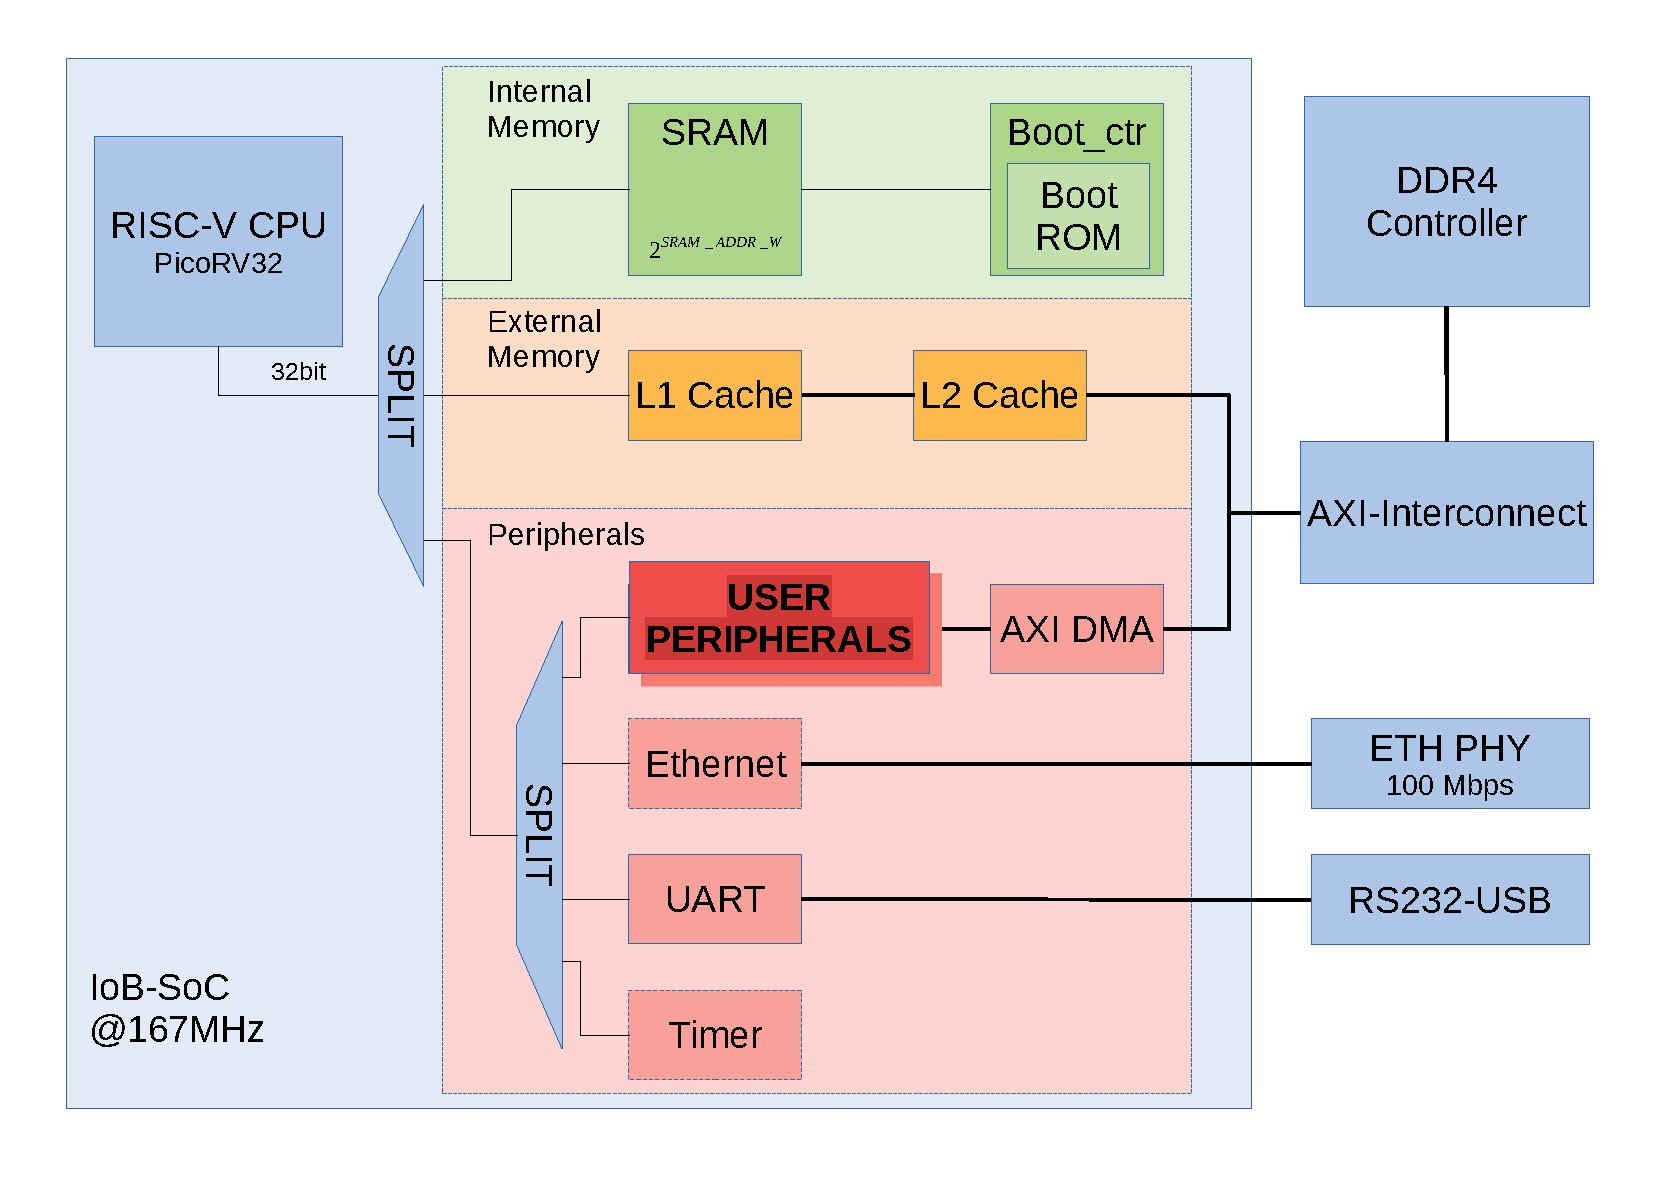
\includegraphics[width=0.7\linewidth]{bd_original.pdf}
    \caption{\textit{IOb-SoC} sketch.}
    \label{fig:bd_original}
\end{figure}

Building a new processor-based system from scratch can be difficult. The \textit{IObundle} developers created the \textit{IOb-SoC} to facilitate this process. This work develops a variant of the existing \textit{IOb-SoC} capable of running a Linux Operating System. \textit{IOb-SoC} currently supports two FPGA board models: the Xilinx Kintex UltraScale KU040 Development Board and the Cyclone V GT FPGA Development Kit.

\subsection{\textit{IOb-SoC} \textit{Makefiles}}
\textit{Makefiles} are essential because they allow automating processes. This way, instead of executing multiple lines to achieve a goal, the user can run a single command. That command will execute a \textit{Makefile} script that runs the multiple processes needed to achieve a specific goal without specifying them. For example, to run a simulation, a developer using this project \acrshort{soc} would only have to write in the terminal the commands in listing~\ref{lst:run_simulation}.

\begin{lstlisting}[language=make, caption={Run a simulation.}, label=lst:run_simulation]
    make sim-clean
    make sim-run
\end{lstlisting}

The first command in listing~\ref{lst:run_simulation} cleans all the files related to a previous simulation execution. Then the second command runs a new simulation. This simulation will use the default configurations in the \enquote{config.mk} file. A \textit{Makefile} target follows each of the \enquote{make} commands. A target is a section of the \textit{Makefile} that may or may not depend on other targets and executes a sequence of commands. In the example~\ref{lst:run_simulation} there are two targets, \enquote{sim-clean} and \enquote{sim-run}.

The main \textit{Makefile} in \textit{IOb-SoC} is located at the \textit{IOb-SoC} root directory. The main \textit{Makefile} contains targets that call other \textit{Makefiles} and sets the values for the default frequency, baud rate, \acrshort{fpga} board used and simulator used. The \textit{Makefiles} the main one can call are at the \textit{IOb-SoC} \acrshort{fpga} boards, simulators, firmware, \enquote{PC} emulation or documentation directory. Each directory in \textit{IOb-SoC} contains a \enquote{*.mk} file which holds \enquote{make} variables and targets that complement the \textit{Makefiles}. The \textit{IOb-SoC} \textit{Makefiles} can include only the \enquote{*.mk} they need.

When executing the command \lstinline[language=bash]{make sim-run} the computer will run the \enquote{run} target of the \textit{Makefile} in the default simulator directory. The simulator \textit{Makefile} will include the \enquote{simulator.mk}, \enquote{hardware.mk} and \enquote{config.mk} files. The \enquote{simulator.mk} file is common to all simulators. Both \acrshort{fpga}s and simulators \textit{Makefiles} include the \enquote{hardware.mk} file. The \enquote{hardware.mk} file includes all the hardware modules that the \acrshort{soc} uses. Lastly, the \enquote{config.mk} is located at the \textit{IOb-SoC} root directory and all \textit{Makefiles} use it. The \enquote{config.mk} defines the \enquote{make} variables that are important for hardware and software, for example which peripherals the \acrshort{soc} contains.

\subsection{\textit{IOb-SoC} peripherals}
Developers add the \textit{IOb-SoC} peripherals under the submodules directory in the \textit{IOb-SoC} folder. Inside the submodules directory, there exists a folder for each peripheral. Furthermore, the \acrshort{cpu}, the \enquote{iob\_cache} module, the \enquote{iob\_mem} hardware, the \enquote{iob\_axi} interface and the \textit{IOb-Lib}~\cite{iob_lib} repository can also be found in the submodules directory. The \textit{IObundle} engineers developed the \textit{IOb-Lib} submodule for it to contain small generic hardware modules and software script used in \textit{IOb-SoC}.

All the submodules may contain hardware and software components. For each hardware peripheral, the \textit{IOb-SoC} engineers recommend developing a set of bare-metal firmware functions that allow using the peripheral with the \acrshort{soc} without an \acrshort{os}. Since the \textit{IOb-SoC} platform also allows emulating the developed firmware in the user's personal computer, the peripherals should have software functions that emulate its firmware drivers.

The peripheral should have the following \enquote{*.mk} files to integrate it into \textit{IOb-SoC}:
\begin{itemize}
    \item the \enquote{PERIPHERAL\_REPO/hardware/hardware.mk} so the user can add the peripheral hardware modules to the \acrshort{soc}.
    \item the \enquote{PERIPHERAL\_REPO/software/embedded/embedded.mk} allows the user to use the peripheral firmware drivers.
    \item the \enquote{PERIPHERAL\_REPO/software/pc-emul/pc-emul.mk} permits emulating the peripheral behaviour in the user's computer.
\end{itemize}
The developer has to include the \enquote{PERIPHERAL\_REPO/hardware/hardware.mk} file in the \textit{IOb-SoC} \enquote{hardware.mk} file. He can include it by adding \lstinline[language=make]{include $(PERIPHERAL_DIR)/hardware/hardware.mk} to the \textit{IOb-SoC} \enquote{hardware.mk}. In the firmware \textit{Makefile} the develops has to include the peripherals \enquote{embedded.mk} file by adding \lstinline[language=make]{include $(PERIPHERAL_DIR)/software/embedded/embedded.mk} to use the peripheral drivers. Lastly in the \enquote{pc-emul} \textit{Makefile} he has to add \lstinline[language=make]{include $(PERIPHERAL_DIR)/software/pc-emul/pc-emul.mk} to allow the software to emulate the peripheral.

In the \enquote{config.mk} file, located in the \textit{IOb-SoC} repository root, the developer needs to add the \enquote{PERIPHERAL\_REPO} to the \enquote{PERIPHERALS} \enquote{make} variable and create a variable that indicates the peripheral directory. The user should define the variable that indicates the peripheral directory similarly to \lstinline[language=make]{PERIPHERAL_DIR=$(ROOT_DIR)/submodules/PERIPHERAL_REPO}.

The peripheral also needs the following files to be automatically instantiated in the \acrshort{soc} hardware: \enquote{inst\_tb.vh}, \enquote{inst.vh} and \enquote{pio.vh}. The \textit{Makefiles} use the \enquote{inst\_tb.vh} file to add the needed Verilog to the testbench core for the system to simulate. It uses the \enquote{inst.vh} to instantiate the peripheral hardware module in the \textit{IOb-SoC} core. Finally, the \enquote{pio.vh} file contains input and output signals that the \textit{Makefiles} must add to the system core hardware. Those files should be in the \enquote{PERIPHERAL\_REPO/hardware/include} directory. Listing \ref{lst:inst_file} presents an example of the \enquote{inst.vh} contents.

\begin{lstlisting}[language=Verilog, caption={Example of the \enquote{inst.vh} file.}, label=lst:inst_file]
//
// TIMER
//
iob_timer timer
  (
   .clk      (clk),
   .rst      (reset),

   //cpu interface
   .valid(slaves_req[`valid(`TIMER)]),
   .address(slaves_req[`address(`TIMER,`TIMER_ADDR_W+2)-2]),
   .wdata(slaves_req[`wdata(`TIMER)]),
   .wstrb(slaves_req[`wstrb(`TIMER)]),
   .rdata(slaves_resp[`rdata(`TIMER)]),
   .ready(slaves_resp[`ready(`TIMER)])
   );
\end{lstlisting}

\subsection{Internal Buses}
The \textit{IObundle} developers designed the \textit{IOb-SoC} in a way that one master hardware component and multiple slave hardware components exist. To Interconnect the hardware components \textit{IOb-SoC} defines two types of bus, the request bus and the response bus. In \textit{IOb-SoC} the master component is the \acrshort{cpu}. The \acrshort{cpu} sends requests to the internal or external memory and the peripherals through the request buses. After making a request, the \acrshort{cpu} will receive the response through the respective response bus. The \acrshort{cpu} instantiated in the \textit{IOb-SoC} core has the \enquote{cpu\_i\_req}, \enquote{cpu\_d\_req}, \enquote{cpu\_i\_resp} and \enquote{cpu\_d\_resp} signals. The \enquote{cpu\_i\_req} signal serves to fetch instructions from memory, and the \enquote{cpu\_i\_resp} will contain the instruction fetched after a few clock cycles. The \acrshort{cpu} uses the \enquote{cpu\_d\_req} to make data requests to either the memory or a \acrshort{soc} peripheral.

The request bus comprises a valid bit, an address signal, a data signal and a strobe signal. The hardware sets the valid bit to ‘1’ when it wants to execute a request and has already defined the other signals. The address signal indicates the register that the request is targeting. Figure \ref{fig:req_bus} shows how the \textit{IOb-SoC} distributes the signals in the request bus. Furthermore, figure \ref{fig:req_bus} also represents the bits equivalent to each signal when the address width and data width are 32 bits. The address and data width in \textit{IOb-SoC} are 32-bit by default.

\begin{figure}[!h]
    \centering
    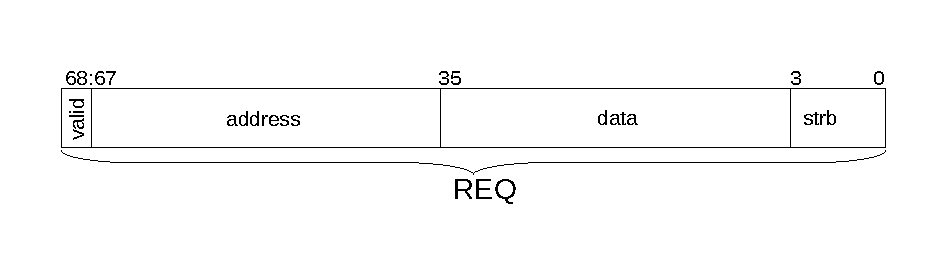
\includegraphics[width=\linewidth]{req_bus.pdf}
    \caption{Request bus with address and data width equal to 32 bits.}
    \label{fig:req_bus}
\end{figure}

The response bus contains a ready bit and a data signal. The hardware sets the ready signal to high when the component that made the request can receive the response. The data signal is the response data to the request made. For example, if the \acrshort{cpu} wants to read the value in a register at address \enquote{x}, the data in the response bus will be the data on register \enquote{x}. Figure \ref{fig:resp_bus} shows how the request signal is composed when the address and data width are 32 bits.

\begin{figure}[!h]
    \centering
    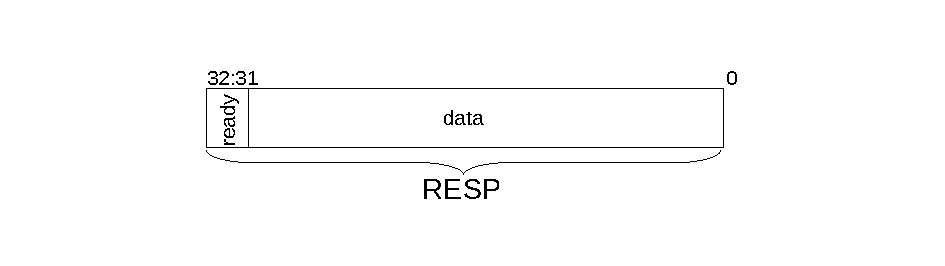
\includegraphics[width=\linewidth]{resp_bus.pdf}
    \caption{Response bus with address and data width equal to 32 bits.}
    \label{fig:resp_bus}
\end{figure}

In the \textit{IOb-Lib} submodule exists a file, called \enquote{iob\_intercon.vh}, that defines a set of macros that can be used in \textit{Verilog}. Developers can use those macros to access the specific bits in the \textit{IOb-SoC} buses. Table \ref{tab:bus_defines} shows the defined macros, how the pre-compiler calculates their value and the respective values when the address and data width are 32-bit.

\begin{table}[!ht]
    \centering
    \begin{tabular}{|l|l|l|l|}
    \hline
    \textbf{Name} & \textbf{Defined expression}          & \textbf{Description}                  & \textbf{\begin{tabular}[c]{@{}l@{}}Value with:\\   ADDR\_W=32\\   DATA\_W=32\end{tabular}} \\ \hline
    READY\_W      & 1                                    & Response ready width                  & 1                                                                                          \\ \hline
    VALID\_W      & 1                                    & Request valid width                   & 1                                                                                          \\ \hline
    WSTRB\_W      & DATA\_W/8                            & Request data width                    & 4                                                                                          \\ \hline
    WRITE\_W      & DATA\_W+DATA\_W/8                    & Most significant bit of request data  & 36                                                                                         \\ \hline
    READ\_W       & DATA\_W+READY\_W                     & Most significant bit of response data & 33                                                                                         \\ \hline
    WDATA\_P      & DATA\_W/8                            & Less significant bit of request data  & 4                                                                                          \\ \hline
    ADDR\_P       & DATA\_W+DATA\_W/8                    & Less significant bit of request data  & 36                                                                                         \\ \hline
    VALID\_P      & ADDR\_W+DATA\_W+DATA\_W/8            & Request bus valid bit position        & 67                                                                                         \\ \hline
    REQ\_W        & VALID\_W+ADDR\_W+WRITE\_W            & Request bus width                     & 69                                                                                         \\ \hline
    RESP\_W       & DATA\_W+READY\_W                     & Response bus width                    & 33                                                                                         \\ \hline
    req(I)        & I*REQ\_W +: REQ\_W                   & Request bus bits boundary             & I*69 +: 69                                                                                 \\ \hline
    resp(I)       & I*RESP\_W +: RESP\_W                 & Response bus bits boundary            & I*33 +: 33                                                                                 \\ \hline
    valid(I)      & I*REQ\_W+VALID\_P                    & Request valid bit position            & I*69+1                                                                                     \\ \hline
    address(I,W)  & I*REQ\_W+ADDR\_P+W-1 -: W            & Request address bits boundary         & I*69+W+35 -: W                                                                             \\ \hline
    wdata(I)      & I*REQ\_W+WDATA\_P +: DATA\_W         & Request data bits boundary            & I*69+4 +: 32                                                                               \\ \hline
    wstrb(I)      & I*REQ\_W +: WSTRB\_W                 & Request strb bits boundary            & I*69 +: 4                                                                                  \\ \hline
    write(I)      & I*REQ\_W +: WRITE\_W                 & Request write bits boundary           & I*69 +: 36                                                                                 \\ \hline
    rdata(I)      & I*RESP\_W+READY\_W +: DATA\_W        & Response data bits boundary           & I*33+1 +: 32                                                                               \\ \hline
    ready(I)      & I*RESP\_W                            & Response ready bit position           & I*33                                                                                       \\ \hline
    \end{tabular}
    \caption{Bus interconnect macros.}
    \label{tab:bus_defines}
\end{table}

Understanding the interconnect macros is essential when developing the interface with peripherals and hardware components for the \textit{IOb-SoC}. Some macros depend on an \enquote{I} value given to them when using the macro. The hardware uses the  \enquote{I} value to distinguish which request or response signal the developers want to access when there is a bus (i.e. wire) with multiple requests or responses. In the \enquote{address(I,W)} macro, the \enquote{W} value corresponds to the number of bits of the address in the request signal the developer wants to select.

\subsection{\textit{iob-split} and \textit{iob-merge}}
The \textit{iob-split} and the \textit{iob-merge} hardware modules can both be found in the \textit{IOb-Lib} submodule hardware directory. The \textit{IOb-SoC} uses the \textit{iob-split} in the systems core and in the internal memory hardware modules. The \textit{iob-split} in \textit{IOb-SoC} separates one request and one response bus into multiple buses and only enables the needed one. For example, there are multiple peripherals; each has an input request bus and an output response bus. However, there is only one \enquote{cpu\_d\_req}. The \textit{iob-split} only sends the \enquote{cpu\_d\_req} signal to the selected peripheral and sets the other peripherals request bus to zeros. The \textit{IOb-SoC} instantiates the \textit{iob-merge} in the external and internal memory hardware modules. The \textit{iob-merge} unifies multiple request and response buses into one. For example, the \acrshort{cpu} can execute both instructions and data requests to the memory. Nevertheless, the memory can only process one request at a time. The \textit{iob-merge} merges the \enquote{cpu\_i\_req} and the \enquote{cpu\_i\_req} and sends to the memory the request with higher priority or the one that was first set has valid.

The \textbf{\textit{iob-split}} is simply a configurable \acrfull{demux}. The developer can configure it when he instantiates the \textit{iob-split} hardware module. The developer can change the size of the \acrlong{demux} and the selection bits through N\_SLAVES and P\_SLAVES, respectively. N\_SLAVES corresponds to the number of slaves. Developers can also interpret N\_SLAVES as the number of the \acrshort{demux} outputs. P\_SLAVES indicates the slave select word \acrfull{msb} position. In other words, P\_SLAVES is the position of the \acrshort{msb} of the \acrlong{demux} selection bits. Equation \ref{eq:number_bits} calculates the number of the selection bits.

\begin{equation}
    \label{eq:number_bits}
    Nb = log_2(N\_SLAVES)+(log_2(N\_SLAVES)==0)
\end{equation}

The \textbf{\textit{iob-merge}} works similar to the \textit{iob-split} but instead of being a \acrshort{demux} it is a configurable \acrfull{mux}. Meaning that instead of having multiple outputs and one input, it has multiple inputs and one output. N\_SLAVES indicates the number of inputs, and P\_SLAVES chooses the selection bits.

\subsection{Bootloader}
The \textit{IObundle} engineers developed a bootloader for \textit{IOb-SoC} that is the first firmware to run on the \acrlong{soc}. The \textit{IOb-SoC} always saves the bootloader firmware in the \acrshort{soc} internal memory in a boot control hardware unit. The boot control hardware unit defines the boot signal. The boot signal is one bit that can be set to high ('1') or low ('0') and indicates whether the \acrshort{soc} should execute the bootloader or other firmware. Moreover, the boot control unit sends a reset signal to the \acrshort{cpu} when the bootloader ends before starting the users' firmware.

Figure \ref{fig:boot_flow} represents a flow chart of the bootloader firmware behaviour. The bootloader starts by initialising the \acrshort{uart} hardware which the \acrshort{soc} uses to communicate with the user's computer. Then it will send an \acrfull{enq} if it still has not sent one. The \acrshort{enq} byte has the value of 0x05 in \acrshort{ascii} and is sent to the user's computer to indicate that the \textit{IOb-SoC} is waiting for the user's computer. The bootloader will ensure the \acrshort{uart} is sending the \acrshort{enq} byte while the user's computer does not send a response. After receiving a response byte, the bootloader firmware checks if the received byte is an \acrfull{frx}. The \acrshort{frx} Byte has the value 0x07. If the bootloader receives a \acrshort{frx}, it has to transfer the firmware that runs after it.

\begin{figure}[!h]
    \centering
    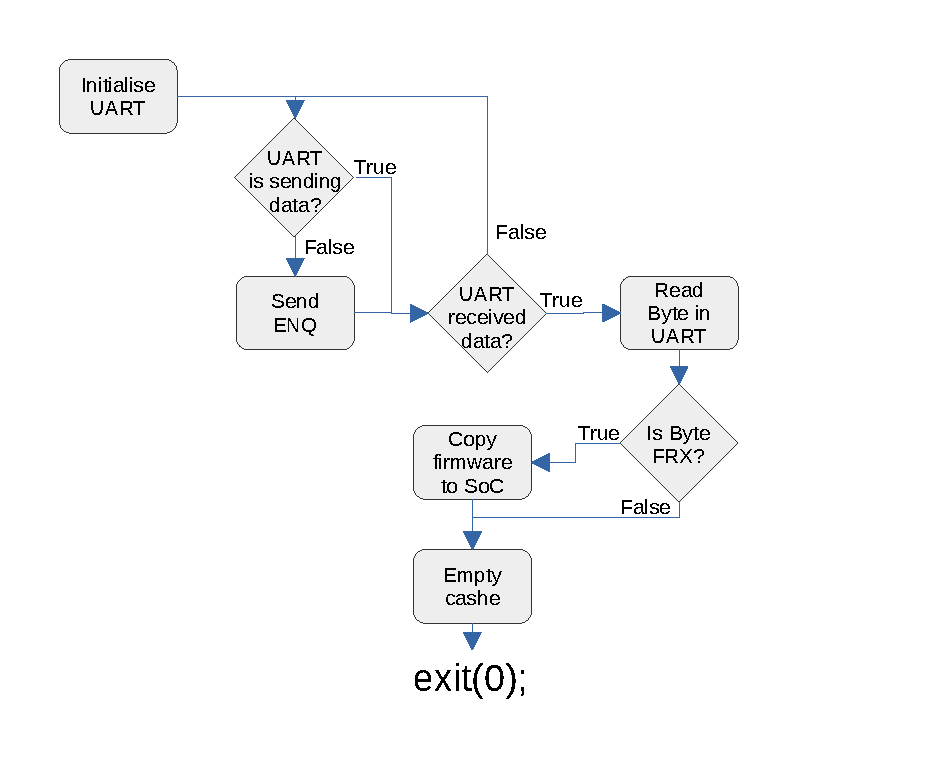
\includegraphics[width=\linewidth]{boot_flow.pdf}
    \caption{Bootloader firmware flow chart.}
    \label{fig:boot_flow}
\end{figure}

When transferring the firmware, the bootloader receives the binary data through the \acrshort{uart} and copies it to the \acrshort{soc} memory. The bootloader can copy the firmware to either the internal or external memory depending on where the user defined the program would be stored. After copying the firmware to the \textit{IOb-SoC}, the bootloader will send the data saved in the memory back to the user's computer. The user's computer can then check if the \textit{IOb-SoC} successfully transferred the firmware by comparing the original firmware binary with the received copy. Before exiting, the bootloader will clean the cache so that the next firmware does not fetch data previously in the cache. Finally, when exiting, the bootloader asks the boot control unit to set the boot signal to low and reset the \acrshort{cpu}.

\section{\textit{RISC-V}}
\label{section:riscv}
\textit{RISC-V}~\cite{asanovic2014instruction} is a free, open-source RISC Instruction Set Architecture (ISA). An ISA is the bridge that connects software and hardware. RISC is one possible classification of the computer ISA's; it means reduced instruction set computer, and the essence of this approach is the simplicity of the instructions computed by the CPU. Unlike a Complex Instruction Set Computer (CISC) ISA, the CPU might have to execute a more significant number of instructions with a RISC ISA to obtain the same result. Since the instructions are simple, more instructions need to be run to complete a given task. However, the architecture is lighter and can run at a higher frequency, compensating for executing more instructions.

The \textit{RISC-V} was initially designed at the University of California, Berkeley. Furthermore, it is called \textit{RISC-V} because it is the fifth RISC instruction set architecture to come out of that university. It was created to support computer architecture research and education. Although now \textit{RISC-V} is used on commercial projects as well. A key advantage of \textit{RISC-V} is its flexibility. It can be used from high-performance computers to deeply embedded systems with no MMU. There exists a 32, 64 and 128-bit version of \textit{RISC-V}. In this report, the 32 and 64-bit versions will be discussed. On the work developed during the thesis preferentially, the 32-bit version will be used. If an instruction is not on the standard \textit{RISC-V}, it can be created as an ISA extension, which provides excellent flexibility.

There are two main parts of the \textit{RISC-V} ISA. There are the \textit{unprivileged} instructions that correspond to the base ISA~\cite{riscv_unpriviledge}, which is composed of only 32-bit instructions and some unprivileged extensions. {Unprivileged instructions} are the instructions that can be used on all privilege modes in all privilege architecture. Moreover, there exists the privilege instructions~\cite{riscv_priviledge} that implements support for the three different privilege levels. Machine mode is the most trusted privilege level, and typically what runs in this mode has low-level access to the machine implementation. The other two modes are the User mode, where most common applications run, and the OS's Supervisor mode. Each privileged mode has its extensions to the ISA.

To install the \textit{RISC-V} tool chain the user can clone their repository and make the necessary cross-compilers. To work with the IOb-SoC, the user will have to install the Newlib cross-compiler. For this work and the development of the thesis, the Linux cross-compiler had to be installed.

Talk about the 32 registers in the register file

The instruction each ISA extension contains...

\acrfull{csr} needed to run a full feature OS... (core\_id, misa, mcause, ...)

\subsection{CLINT Specification}
\label{subection:clint_riscv}
The \textit{RISC-V} \textbf{CLINT} is described ...
Platform must support an ACLINT MTIME counter resolution of 100ns or less (corresponding to a clock tick frequency of at least 10 MHz).

\subsection{PLIC Specification}
\label{subection:plic_riscv}
The \textit{RISC-V} \textbf{PLIC} was first described in the privilege instructions documentation, but since version 1.10 it was moved to its own document.

\subsection{UART/Serial Console}
\label{section:serial_console}
In the \textit{RISC-V} Platform Specification~\cite{riscv_platform_specification} it is defined that every embedded \acrfull{os} is required to have a \acrshort{uart} port implementation that is register-compatible with the industry standard \textit{UART 16550}. The \textit{UART 16550} already exists for a long time, it was released by \textit{National Semiconductor} in 1987, and is present and supported by a large number of software and hardware. The \textit{UART 16550} is often used connected to an RS-232 interface. The \textit{IOb-SoC} supported development boards are connected through RS-232 to the computer.

The \textit{UART 16550} registers are...
\begin{table}[!ht]
    \centering
    \begin{tabular}{|l|l|l|l|l|}
    \hline
    \textbf{Name}                      & \textbf{Address} & \textbf{Width} & \textbf{Access} & \textbf{Description}                                                                    \\ \hline
    Receiver Buffer                    & 0                & 8              & R               & Receiver FIFO output                                                                    \\ \hline
    Transmitter Holding Register (THR) & 0                & 8              & W               & Transmit FIFO input                                                                     \\ \hline
    Interrupt Enable                   & 1                & 8              & RW              & \begin{tabular}[c]{@{}l@{}}Enable/Mask interrupts\\  generated by the UART\end{tabular} \\ \hline
    Interrupt Identification           & 2                & 8              & R               & Get interrupt information                                                               \\ \hline
    FIFO Control                       & 2                & 8              & W               & Control FIFO options                                                                    \\ \hline
    Line Control Register              & 3                & 8              & RW              & Control connection                                                                      \\ \hline
    Modem Control                      & 4                & 8              & W               & Controls modem                                                                          \\ \hline
    Line Status                        & 5                & 8              & R               & Status information                                                                      \\ \hline
    Modem Status                       & 6                & 8              & R               & Modem Status                                                                            \\ \hline
    \end{tabular}
    \caption{Normally assessed \textit{\acrshort{uart}16550} registers.}
    \label{tab:uart16550_regs}
\end{table}

\begin{table}[!ht]
    \centering
    \begin{tabular}{|l|l|l|l|l|}
    \hline
    \textbf{Name}              & \textbf{Address} & \textbf{Width} & \textbf{Access} & \textbf{Description}                                                                      \\ \hline
    Divisor Latch Byte 1 (LSB) & 0                & 8              & RW              & \begin{tabular}[c]{@{}l@{}}The less significant Byte\\  of the divisor latch\end{tabular} \\ \hline
    Divisor Latch Byte 2 (MSB) & 1                & 8              & RW              & \begin{tabular}[c]{@{}l@{}}The most significant Byte\\  of the divisor latch\end{tabular} \\ \hline
    \end{tabular}
    \caption{Divisor latch \textit{\acrshort{uart}16550} registers.}
    \label{tab:uart16550_divisor_regs}
\end{table}

Finally when using 32-bit data bus interface, there are two additional registers for debugging. The first register address is 8 and the second is 12. Both registers are 8 bits and read only.

\subsection{The Linux Boot Flow}
\label{subection:linux_boot_flow}
What is a device tree?

\subsection{OpenSBI}
\label{subection:opensbi}
Talk SBI!

\section{Open Source Verification tools}
\label{section:verification_tools}
Verification tools are ....

Other emulators are Trace-accurate, like Spike, and Cycle-accurate, for example, Verilator. 

https://www.sifive.com/blog/risc-v-qemu-part-1-privileged-isa-hifive1-virtio

\subsection{Hardware logic simulators}
It is important to have a good hardware simulation environment for testing purposes. Researchers take advantage of already existing and well-developed tools. Several simulation tools exist, most of which are proprietary, for example, \textit{xcelium} from \textit{Candence}. Its utilisation can increase the cost of a project significantly. In this thesis, we will use open-source, free-to-use verification tools. In specific, we will take advantage of \textit{Icarus Verilog}~\cite{williams2006icarus} and \textit{Verilator}~\cite{snyder2010verilator}. Although both tools are for verification, they serve different purposes due to their characteristics.

\begin{itemize}
    \item \textbf{\textit{Icarus Verilog}} is a Logic Simulator that uses Verilog or System-Verilog testbench to test the UUT (Unit Under Test). Unfortunately, its support for System-Verilog is limited, and some designs might not run in this simulator. \textit{Icarus Verilog} is also known as \textit{IVerilog}.
    
    After compiling the hardware design, \textit{IVerilog} outputs a file which can be run line by line to simulate the designed logic.
    
    \item \textbf{\textit{Verilator}} transforms the \textit{Verilog} \acrshort{hdl} designs into a \textit{C++} program that can be executed after being compiled. Using \textit{C++} to create a testbench allows calling the converted hardware program as a function of a normal \textit{C++} library. Executing the \textit{C++} testbench simulates the hardware initially described in \textit{Verilog}. While also allowing to make use of system calls easily. The testbench needed to run with Verilator is similar to the testbench in \textit{Verilog} used with \textit{IVerilog}.
\end{itemize}

\textbf{The biggest differences} are: \textit{Verilator} only represents logic signal as 1's or 0's, contrary to \textit{IVerilog} which also represents unknown values as X's; Since \textit{Verilator} ends up being a C++ program it is much faster to run the simulation than with \textit{IVerilog}; On another perspective \textit{Verilator} is slower than \textit{IVerilog} to interpret the hardware logic design.
As such, it is easier to use \textit{IVerilog} to detect errors in the design, but it is better to use \textit{Verilator} for more complex simulations.

\subsection{\textit{QEMU} Simulation}
\textit{QEMU}~\cite{bellard2005qemu} is an open-source machine emulator and virtualiser that allows running software and firmware, like operating systems, on many different devices and architecture using a personal computer. \textit{QEMU} is similar to \textit{VMware}~\cite{bugnion2012bringing} or \textit{VirtualBox}~\cite{oracle2015virtualbox}. \textit{VMware} and \textit{VirtualBox} allow the user to create virtual machines that simulate real hardware and execute an operating system. Developers can use \textit{QEMU} to run an operating system on virtual hardware.

\textit{QEMU} is considered a functional emulator; it translates the instructions that were supposed to run on the target architecture to instructions that run on the host CPU. The advantage of using a functional emulator like \textit{QEMU} is that it is way faster than the other emulation types. A functional emulator runs 100 million to > 1 billion instructions per second, while trace-accurate or cycle-accurate run 10 to 100 thousand instructions per second.

\textit{QEMU} can be used to emulate both 32-bit and 64-bit \textit{RISC-V} CPUs. \textit{QEMU} is ideal for testing user applications written to execute on a \textit{RISC-V} embedded system. User applications, contrary to the initial bootloaders, are platform-independent. In case of an application not running on a certain \acrshort{soc}, developers can use \textit{QEMU} to check if the problem is the application or the \acrshort{soc}. A user can emulate an operating system by compiling the firmware to be compatible with the \textit{QEMU} \enquote{virt} board. The \enquote{virt} is a board that does not replicate any actual hardware. However, the \textit{QEMU} developers designed this virtual hardware so the users could test the software even if there existed no hardware that could run it. To define which board the emulation is supposed to run in when calling \textit{QEMU}, the user should pass \textit{--machine virt} as an argument.

\chapter{Existing Embedded Technologies}
\label{chapter:existing_embedded_technologies}
There already exists embedded microcontrollers capable of running Linux. Big companies for example ARM, Qualcomm, MediaTek, Intel and AMD have created microcontrollers capable of running Linux. But the processor architecture of those microcontrollers is not open-source, much less the microcontroller itself.

As an example, the \textit{Raspberry Pi 4} is a very capable and cheap board where a developer can test and implement new software running in Linux. The Raspberry \acrshort{cpu} is an \textit{Cortex-A72}~\cite{cortex_a72} witch is a System on Chip (SoC) developed by ARM on their ARMv8 64-bit CPU architecture. But if someone wanted to use the Raspberry as a base for his costume hardware design, that would be impossible. And thus appears the need for open-source hardware that allows creating something new without having to start from scratch every time. This led to the appearance of \textit{RISC-V} the open-source CPU architecture.


\section{Closed source \textit{RISC-V} Embedded Systems}
\label{section:closed_source}
Since then, a few companies using \textit{RISC-V} have appeared. \textit{RISC-V} CPUs are already present in the automotive and IoT markets, besides AI chips in data centres. Due to the \textit{RISC-V} ISA royalty-free license, new StartUps tend to look at \textit{RISC-V} CPUs as a solution for their cores. Even if the CPU Core isn't free to use it ends up being a cheaper solution.

While creating new products companies proved how advantageous the \textit{RISC-V} architecture was. Furthermore, they have contributed to open-source software, hardware and documentation. Some companies with big recognition involved with \textit{RISC-V} technology are:
\begin{itemize}
    \item \textit{Western Digital} who now uses \textit{RISC-V} in its external storage disks.
    \item \textit{Microchip} as launched the first \textit{RISC-V}-Based System-on-Chip (SoC) FPGA, \textit{PolarFire}.
    \item \textit{Antmicro/Microsemi}~\footnote{Microchip has acquired Microsemi Corporation in May 2018.} have built a software called Renode that is used to develop, debug and test multi-node \textit{RISC-V} device systems.
    \item \textit{BeagleBoard.org}, \textit{Seeed Studio} and \textit{StarFive} worked together to build the first affordable \textit{RISC-V} computer designed to run Linux, \textit{BeagleV}~\cite{beagleV}. The board is priced around 150€.
\end{itemize}

These companies have all helped pave the way for a full-feature Operating System based on the Linux kernel to be compatible with the \textit{RISC-V} architecture. However, two companies have a bigger impact on \textit{RISC-V} CPU design, those are Andes Technology and SiFive.

\subsection{Andes Technology}
Andes Technology is one of the founding members of \textit{RISC-V} International. Since it is highly involved with \textit{RISC-V} it ended up being one of the major contributors (and maintainers) of the \textit{RISC-V} toolchain. This is important because the \textit{RISC-V} ISA is merely an instruction set architecture, there needs to exist complementing software, such as compiler and development tools.

Nowadays Andes CPUs are applied nearly everywhere, from telecommunications, storage controllers, and touch screen sensors to data centres, etc. Andes Technologies has had incredible success using \textit{RISC-V} technology, as proof they have shipped billions of embedded SoC with \textit{RISC-V} processors based on their \textit{RISC-V} ISA variant, AndeStar™ V5.

Andes CPUs which are capable of running Linux are the \textit{A25}~\cite{a25} and \textit{AX25}~\cite{ax25}. Both support single and double precision floating points, the \textit{RISC-V} P-extension (draft) DSP/SIMD ISA and an MMU (Memory Management Unit) for Linux applications. Besides that both enable the use of Machine (M), User (U) and Supervisor (S) Privilege levels that allow running Linux and other advanced operating systems with protection between kernel and user programs. Furthermore, both have L1 instructions and data cache. The difference between them is that \textit{A25} is based on 32-bit architecture and the \textit{AX25} is 64-bit. This leads to the \textit{AX25} being ideal for embedded applications that need to access address space over 4GB, and the \textit{A25} being smaller in gate count. Both CPUs can be implemented on the AE350~\cite{ae350} SoC allowing to use these CPUs on developer boards, for example in the \textit{ADP-XC7K160/410}~\cite{adp-xc7k160}.

\subsection{SiFive}
SiFive is a company that was born from the \textit{RISC-V} ISA. SiFive was founded by three researchers from the University of California Berkeley, Krste Asanović, Yunsup Lee, and Andrew Waterman. Those researchers were deeply involved with the development of the \textit{RISC-V} ISA, from working on the base ISA to working on the floating point numbers and compressed instructions ISA extensions. It is no surprise that the first company to release a chip and development board that implemented the \textit{RISC-V} ISA was SiFive. This happened in 2016 one year after the company was founded.

In 2017 SiFive launched \textit{U54}~\cite{u54} which was the first \textit{RISC-V} CPU capable of running a full fledge Operating System like Linux. With it they launched the \textit{U54-MC}~\cite{u54-mc} SoC that had four \textit{U54} 64-bit cores. Furthermore, the \textit{U54-MC} implemented the initial CLINT and PLIC unit. The development of the \acrshort{clint} and the \acrshort{plic} made by SiFive would eventually lead to the documentation and specification of the respective hardware components with which \textit{RISC-V} systems must be compliant if they proclaim to use either one. One year after, in 2018, they launched \textit{HiFive Unleashed}~\cite{hifive_unleashed} which was the first board that implemented the \textit{U54} CPU and run a Linux OS with a desktop environment (DE). The \textit{HiFive Unleashed} has been discontinued and better hardware has been made available.

SiFive has since then extended its \textit{U Cores} product lineup. All \textit{U} cores are 64-bit application processors capable of running Linux. The highest performance core is the \textit{U74}~\cite{u74}. The core architecture is RV64GBC which means it supports the \textit{RISC-V} I, M, A, F, D, B and C ISA extensions (explained in \textbf{*ref section 2.3.x*}). This CPU has already been applied to multiple boards, for example, the \textit{BeagleV} has a \acrshort{soc} with dual-core SiFive \textit{U74} CPU. SiFive as also launched its own development board, \textit{HiFive Unmatched}~\cite{hifive_unmatched}, with four \textit{U74} cores on the \textit{U74-MC}~\cite{u74-mc} SoC. Furthermore, in 2021, Canonical the developers behind Ubuntu announced the OS support for both the HiFive Unmatched and HiFive Unleashed.

\section{Open-Source Solutions}
\label{section:open_source_solutions}
Built upon the \textit{RISC-V} open-source \acrlong{isa}, various CPU designs have emerged. Some of them are fully open-source and might be implemented in other projects. Those CPUs were mostly developed by Universities research groups or by individuals with a grant.

\textit{RISC-V} CPUs are most popular in embedded systems and IoT devices. Consequently there exists a wide variety of open-source CPUs which are implemented on multiple embedded microcontrollers. A few examples of those \acrshort{cpu}s would be the \textit{PicoRV32}~\cite{picorv32}, \textit{NEORV32}~\cite{neorv32}, \textit{DarkRISCV}~\cite{darkriscv} and \textit{Ibex}~\cite{ibex} from lowRISC. But those will not be discussed in detail in this paper since they do not meet the requirements to run the Linux Kernel. This \acrshort{cpu}s either only support \acrfull{machine} level privilege mode or support \acrfull{machine}+\acrfull{supervisor} mode. Moreover, none of the given examples supports the Atomic \textit{RISC-V} \acrshort{isa} extension. This extension is essential to run Linux. Since the kernel explicitly executes instructions from the Atomic extension.

To run a Linux-based Operating System an application processor is needed. A \acrshort{cpu} is considered an \textit{application processor} if it has the hardware required to run a full-feature \acrfull{os} and user applications. This means that the processor should have the required \acrfull{csr}, support \acrshort{machine}+\acrshort{supervisor}+\acrshort{user} privilege modes and support atomic instructions. An open-source solution would be either the \textit{CVA6}~\cite{zaruba2019cost} (previously known as Ariane), \textit{BOOM}~\cite{zhaosonicboom} or \textit{VexRiscv}~\cite{vexriscv}.

\subsection{\textit{CVA6}}
The CVA6 is a 6-stage, single issue, in-order CPU which can execute either the 32-bit or 64-bit \textit{RISC-V} instruction set. CVA6 has support for the I, M, A and C \textit{RISC-V} \acrshort{isa} extensions. The original design was initiated in a research group by a PhD student at ETH Zurich (where they called the core Ariane). Since then the development and maintenance of CVA6 were incorporated in the \textit{OpenHW Group} as part of their CORE-V processor lineup. The support for RV32IMAC was only developed recently by Thales and is also open-source. The \acrshort{cpu} design is illustrated in figure \ref{fig:cva6_design} that was obtained from: \url{https://github.com/openhwgroup/cva6/}.

\begin{figure}[!h]
    \centering
    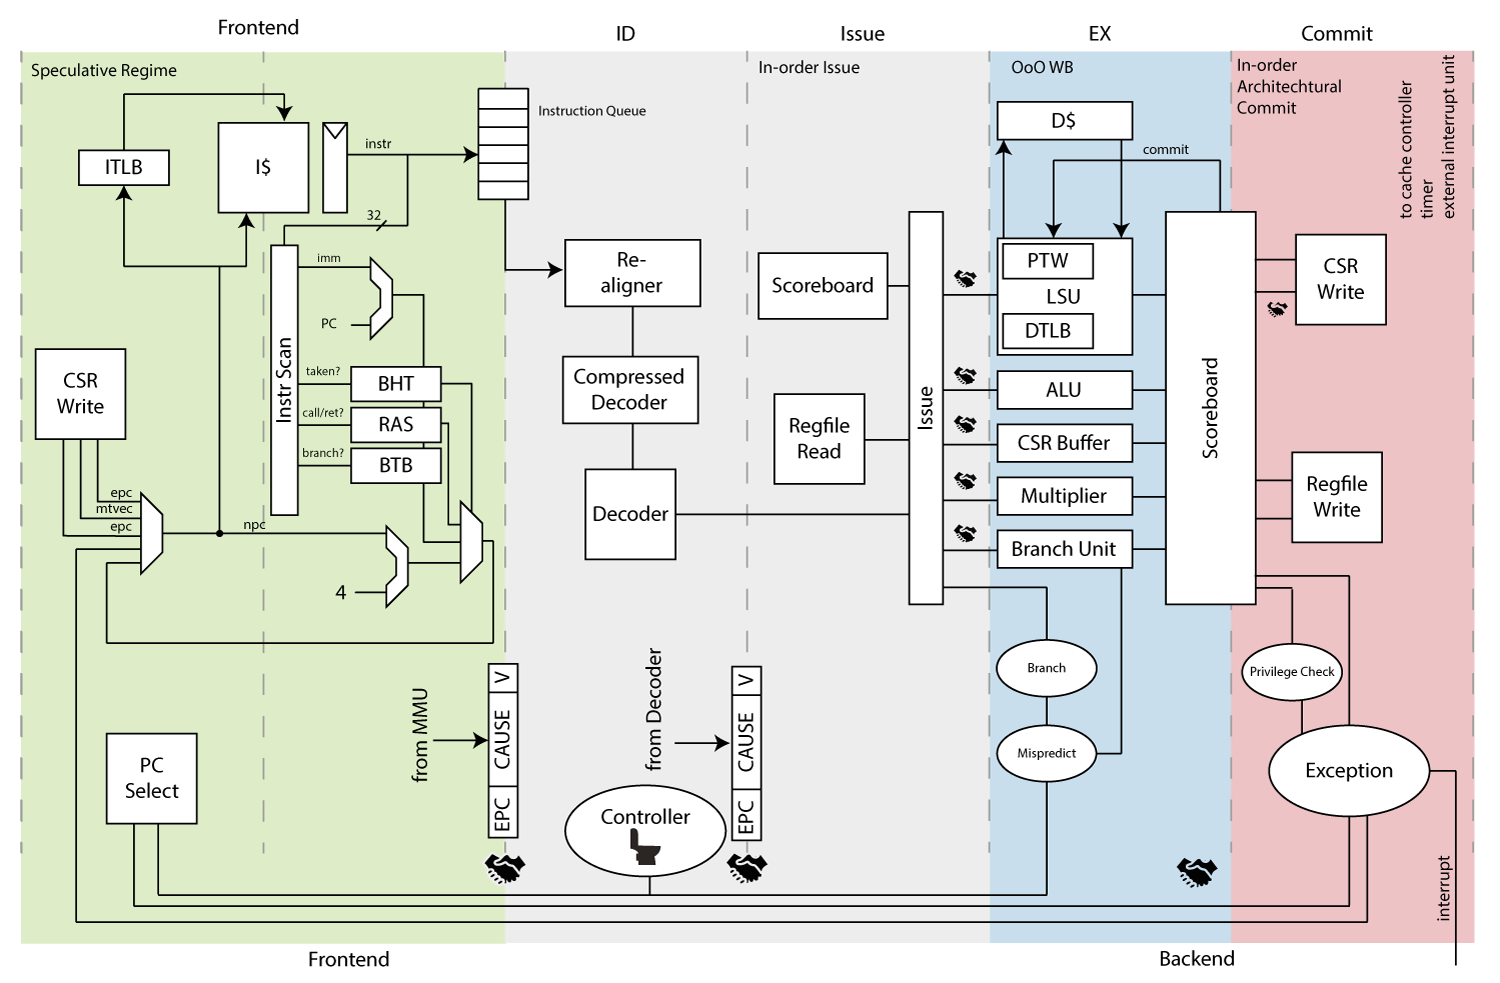
\includegraphics[width=0.7\linewidth]{cva6_design.png}
    \caption{CVA6 core design architecture.}
    \label{fig:cva6_design}
\end{figure}

The CVA6 supports any operating system based on Unix since it implements the three needed privilege levels M, S and U. The core is written in SystemVerilog, and its micro-architecture is designed to reduce the critical path length. Since it is written in SystemVerilog, it is easier for someone knowledgeable in the classic Verilog and VHDL languages to understand and create a customized CPU based on the CVA6, than if it was written in a high-level hardware description language. However, although the CVA6 is an open-source project it is hard to take advantage of isolated hardware components. This is a consequence of how it was developed. Every SystemVerilog module of the CVA6 depends on other files from the project and the CPU itself is very little customizable. To illustrate the problem if we wanted to remove the L1 cache present in the CVA6 to use the L1 cache used on IOb-SoC, it would be very difficult and time-consuming to create a CPU core without that component.

The CVA6 can be found implemented on \textit{OpenPiton}~\cite{Balkind:2016:OOS:2872362.2872414}. \textit{OpenPiton} is an open-source project developed by the Princeton Parallel Group. With it, one can easily create an SoC that has multiple CV6 cores and run a full-feature \acrfull{os} on a development board with an FPGA.

\subsection{The Berkeley Out-of-Order \textit{RISC-V} Processor}
The Berkeley Out-of-Order \textit{RISC-V} Processor (\textit{BOOM}~\cite{zhaosonicboom}) is a superscalar \acrfull{ooo} processor executing the RV64GC variant of the \textit{RISC-V} ISA. BOOM was created at the University of California, Berkeley in the Berkeley Architecture Research group. The CPU design is optimized to run on ASICs, although it can also be implemented on FPGAs. Its priority is to be a high-performance, synthesizable, and parametrizable core for architecture research. The current release, named \textit{SonicBOOM}, has one of the best performances from the publicly available open-source \textit{RISC-V} cores.

BOOM is a 10-stage CPU with the following stages: Fetch, Decode, Register Rename, Dispatch, Issue, Register Read, Execute, Memory, Writeback, and Commit. However, in most practical implementations, many of those stages are merged, generating seven stages altogether: Fetch, Decode/Rename, Rename/Dispatch, Issue/Register Read, Execute, Memory and Writeback. Since committing happens asynchronously, it is not counted as part of the \enquote{pipeline}. The load-store unit is optimized for the superscalar out-of-order architecture, and the data cache is organized into two dual-ported banks. At the front end, it is possible to customize the size of the L1 Instruction cache, the TLB, and the decode stage. Similarly to the CVA6, it is difficult or impossible to remove the cache from the core design and use the IOb-Cache instead.

This \acrshort{cpu} design is written in Chisel~\cite{bachrach2012chisel} \acrfull{hdl}. The \acrfull{chisel} allows for the production of synthesizable Verilog designs while using a high-level language to describe the hardware. \acrshort{chisel} is an adaptation of Scala~\cite{odersky2004scala} programing language, adding hardware construction primitives.

To build a \acrfull{soc} with BOOM we would have to utilize the \textit{Rocket Chip}~\cite{asanovic2016rocket} SoC generator from CHIPS Alliance. Since BOOM uses micro-architecture structures (TLBs, PTWs, etc) from that tool.

\subsection{\textit{VexRiscv}}
The \textit{VexRiscv}~\cite{vexriscv} CPU is a 32-bit Linux Capable \textit{RISC-V} CPU written in the \textit{SpinalHDL}~\cite{papon2017spinalhdl}. The hardware description of this CPU is accomplished by utilizing a software-oriented approach. Similarly to \acrshort{chisel}, \textit{SpinalHDL} is based on the Scala programing language.

VexRiscv is an in-order CPU with five \enquote{pipeline} stages. Many CPU plugins are optional, which add many functionalities to build a custom \textit{RISC-V} CPU. The architecture design approach in this processor is unconventional, but it has its benefits: there are remarkably few fixed hardware components; Parts of the CPU can be swapped, turned on and turned off via the plugin system; without modifying any of the CPU sources, it is possible to add new functionalities/instructions easily; It permits the CPU arrangement to cover a significantly large spectrum of implementations, allowing the construction of an entirely parametrized CPU design. When the CPU is configured without plugins, it only includes the description of the five \enquote{pipeline} stages and their basic functionalities and nothing else. Everything else needs to be added to the CPU via plugins, including the program counter. VexRiscv can either be an application processor capable of running a full-feature \acrfull{os} or a super simple microprocessor ideal for bare-bone applications depending on the way it is configured. Contrary to \textit{BOOM}, \textit{VexRiscv} does not need any external library. This makes it very easy to generate the synthesizable Verilog file from a \textit{SpinalHDL} design.

There exists an open-source project that runs Linux with \textit{VexRiscv}, \textit{linux-on-litex-vexriscv}~\cite{litex_vexriscv}. \textit{LiteX} is used to create a \acrfull{soc} around the \textit{VexRiscv} core. \textit{LiteX} \acrshort{soc} design and peripherals are written in \textit{Migen}~\cite{bourdeauducq2012migen} another high level \acrshort{hdl}. \textit{Migen} unlike \textit{SpinalHDL} and  \acrshort{chisel} is based on Python 3.5. On account of the language describing its hardware and the way, the \textit{linux-on-litex-vexriscv} project is structured it is very hard to understand how the system works, where the generated \acrshort{rtl} is and how to add custom hardware. Furthermore, \textit{linux-on-litex-vexriscv} uses \acrshort{fpga} specific hardware, making it impossible to port the system to \acrshort{asic}.

Recently the developer behind \textit{SpinalHDL} has also made public the \textit{NaxRiscv} \acrshort{cpu}. \textit{NaxRiscv} is a \acrshort{cpu} designed specifically to run a full-feature \acrlong{os}, like Linux. And just like \textit{VexRiscv}, \textit{NaxRiscv} uses \textit{SpinalHDL} to describe its hardware. Although \textit{NaxRiscv} seems like a very promising \acrshort{cpu} it is still on its early stages. Consequently, it has a primitive interface which makes it complicated to implement on costume \acrfull{soc}.


\section{Overall CPU comparison}
\label{section:cpu_comparison}
In table \ref*{tab:cpu_comparison} we can see a comparison of the \acrshort{cpu}s that were presented in the previous sections, capable of running a full-feature \acrfull{os}. All of the CPUs on the table are considered application processors. It can be observed that every CPU has a \acrfull{mmu} and they all support \acrshort{user}+\acrshort{supervisor}+\acrshort{machine} privilege mode. Furthermore, all of the \acrshort{cpu}s hardware design have L1 Instruction Cache and L1 Data cache system integrated. This happens because to support atomic instructions it is easier to have direct access to the L1 Cache.

\textit{GNU/Linux} is the combinations of \textit{GNU} with the Linux kernel. The GNU Project developed a large part of the software that forms a complete \acrfull{os}. Many \enquote{Linux} distributions make use of that software, a few examples would be \textit{Debian}, \textit{Ubuntu}, \textit{openSUSE}, \textit{Fedora}, and the list could go on. So a processor that supports the GNU/Linux feature is a CPU that is capable of running a distribution like \textit{Ubuntu} or \textit{Debian}. From the table, we can see that 32-bit \textit{RISC-V} \acrshort{cpu}s are the only ones not capable of running a \textit{GNU/Linux} \acrfull{os}.

\begin{table}[!ht]
    \centering
    \resizebox{\textwidth}{!}{%
    \begin{tabular}{cccccccccc}
        & ARM                             & \multicolumn{2}{c}{Andes Technology}                      & \multicolumn{2}{c}{SiFive}                                & PULP platform                 & UC Berkeley                 & \multicolumn{2}{c}{SpinalHDL}                                 \\ \cline{2-10}
\multicolumn{1}{c|}{}                                                                   & \multicolumn{1}{c|}{Cortex-A72} & \multicolumn{1}{c|}{A25}    & \multicolumn{1}{c|}{AX25}   & \multicolumn{1}{c|}{U54}    & \multicolumn{1}{c|}{U74}    & \multicolumn{1}{c|}{CVA6}      & \multicolumn{1}{c|}{BOOM}   & \multicolumn{1}{c|}{VexRiscv} & \multicolumn{1}{c|}{NaxRiscv} \\ \hline
\multicolumn{1}{|c|}{\begin{tabular}[c]{@{}c@{}}Architecture\\ bit widths\end{tabular}} & \multicolumn{1}{c|}{64-bit}     & \multicolumn{1}{c|}{32-bit} & \multicolumn{1}{c|}{64-bit} & \multicolumn{1}{c|}{64-bit} & \multicolumn{1}{c|}{64-bit} & \multicolumn{1}{c|}{32/64-bit} & \multicolumn{1}{c|}{64-bit} & \multicolumn{1}{c|}{32-bit}   & \multicolumn{1}{c|}{64-bit}   \\ \hline
\multicolumn{1}{|c|}{MMU}                                                               & \multicolumn{1}{c|}{Y}          & \multicolumn{1}{c|}{Y}      & \multicolumn{1}{c|}{Y}      & \multicolumn{1}{c|}{Y}      & \multicolumn{1}{c|}{Y}      & \multicolumn{1}{c|}{Y}         & \multicolumn{1}{c|}{Y}      & \multicolumn{1}{c|}{Y}        & \multicolumn{1}{c|}{Y}        \\ \hline
\multicolumn{1}{|c|}{FPU}                                                               & \multicolumn{1}{c|}{Y}          & \multicolumn{1}{c|}{Y}      & \multicolumn{1}{c|}{Y}      & \multicolumn{1}{c|}{Y}      & \multicolumn{1}{c|}{Y}      & \multicolumn{1}{c|}{X}         & \multicolumn{1}{c|}{Y}      & \multicolumn{1}{c|}{X}        & \multicolumn{1}{c|}{Y}        \\ \hline
\multicolumn{1}{|c|}{\begin{tabular}[c]{@{}c@{}}16-bit \\ instructions\end{tabular}}    & \multicolumn{1}{c|}{X}          & \multicolumn{1}{c|}{Y}      & \multicolumn{1}{c|}{Y}      & \multicolumn{1}{c|}{Y}      & \multicolumn{1}{c|}{Y}      & \multicolumn{1}{c|}{Y}         & \multicolumn{1}{c|}{Y}      & \multicolumn{1}{c|}{Y}        & \multicolumn{1}{c|}{X}        \\ \hline
\multicolumn{1}{|c|}{Cache L1(I+D)}                                                     & \multicolumn{1}{c|}{Y}          & \multicolumn{1}{c|}{Y}      & \multicolumn{1}{c|}{Y}      & \multicolumn{1}{c|}{Y}      & \multicolumn{1}{c|}{Y}      & \multicolumn{1}{c|}{Y}         & \multicolumn{1}{c|}{Y}      & \multicolumn{1}{c|}{Y}        & \multicolumn{1}{c|}{Y}        \\ \hline
\multicolumn{1}{|c|}{\begin{tabular}[c]{@{}c@{}}Interrupt \\ Controller\end{tabular}}   & \multicolumn{1}{c|}{X}          & \multicolumn{1}{c|}{Y}      & \multicolumn{1}{c|}{Y}      & \multicolumn{1}{c|}{Y}      & \multicolumn{1}{c|}{Y}      & \multicolumn{1}{c|}{X}         & \multicolumn{1}{c|}{X}      & \multicolumn{1}{c|}{X}        & \multicolumn{1}{c|}{X}        \\ \hline
\multicolumn{1}{|c|}{\acrshort{user}+\acrshort{supervisor}+\acrshort{machine} Mode}                                                        & \multicolumn{1}{c|}{N/A}        & \multicolumn{1}{c|}{Y}      & \multicolumn{1}{c|}{Y}      & \multicolumn{1}{c|}{Y}      & \multicolumn{1}{c|}{Y}      & \multicolumn{1}{c|}{Y}         & \multicolumn{1}{c|}{Y}      & \multicolumn{1}{c|}{Y}        & \multicolumn{1}{c|}{Y}        \\ \hline
\multicolumn{1}{|c|}{GNU/Linux}                                                         & \multicolumn{1}{c|}{Y}          & \multicolumn{1}{c|}{X}      & \multicolumn{1}{c|}{Y}      & \multicolumn{1}{c|}{Y}      & \multicolumn{1}{c|}{Y}      & \multicolumn{1}{c|}{Y}         & \multicolumn{1}{c|}{Y}      & \multicolumn{1}{c|}{X}        & \multicolumn{1}{c|}{Y}        \\ \hline
\multicolumn{1}{|c|}{Open-Source}                                                       & \multicolumn{1}{c|}{X}          & \multicolumn{1}{c|}{X}      & \multicolumn{1}{c|}{X}      & \multicolumn{1}{c|}{X}      & \multicolumn{1}{c|}{X}      & \multicolumn{1}{c|}{Y}         & \multicolumn{1}{c|}{Y}      & \multicolumn{1}{c|}{Y}        & \multicolumn{1}{c|}{Y}        \\ \hline
\end{tabular}%
    }
    \caption{CPU comparison table: Y means the CPU supports the feature; X means the CPU does not support the feature; N/A means the feature does not apply to the respective CPU.}
    \label{tab:cpu_comparison}
\end{table}

\chapter{Hardware Developed}
\label{chapter:hardware_developed}
During the development of this thesis, there was both hardware and software developed. In this chapter, we are going to go through the hardware developed to build an appropriate \acrfull{soc} capable of running a full-fledged \acrfull{os}.

The \textit{IOb-SoC} was used as a \acrfull{soc} template. \textit{IOb-SoC} has some features that make it ideal to develop this project \acrshort{soc}. Firstly, it is open-source hardware. This means there are no royalties and the source code is publicly available. Secondly, adding new peripherals is very easy and intuitive, as was previously seen in section~\ref{section:the_iob_soc_template}. Thirdly, the \textit{IOb-SoC} implements the interface with an internal (SRAM) and an external (DRAM) memory. When using an external memory the \textit{IOb-SoC} instantiates an \textit{iob-cache} system. Finally, the \textit{IOb-SoC} implements a boot hardware unit that controls the first boot stage (also known as stage zero) that is executed after powering/resetting the system.

The hardware components that needed to be changed from \textit{IOb-SoC} were the \acrfull{cpu} and the \acrfull{uart} peripheral. The \acrshort{cpu} had to be changed because the previous \acrshort{cpu} (\textit{PicoRV32}) is not capable of running a full-feature \acrlong{os}. The \acrshort{uart} had to be swapped since there were no compatible Linux drivers that worked with \textit{iob-UART}. Besides swapping a few components from the chip new hardware had to be added. The additional hardware is the \acrshort{clint} and the \acrshort{plic} both compatible with RISC-V specifications. The \acrshort{clint} was added to implement timer and software interrupts on the \acrshort{soc}. The \acrshort{plic} was added to manage interrupts generated by other peripherals, for example from the \acrshort{uart}. A sketch of the \acrshort{soc} developed can be seen in figure \ref{fig:bd_linux}.

\begin{figure}[!h]
    \centering
    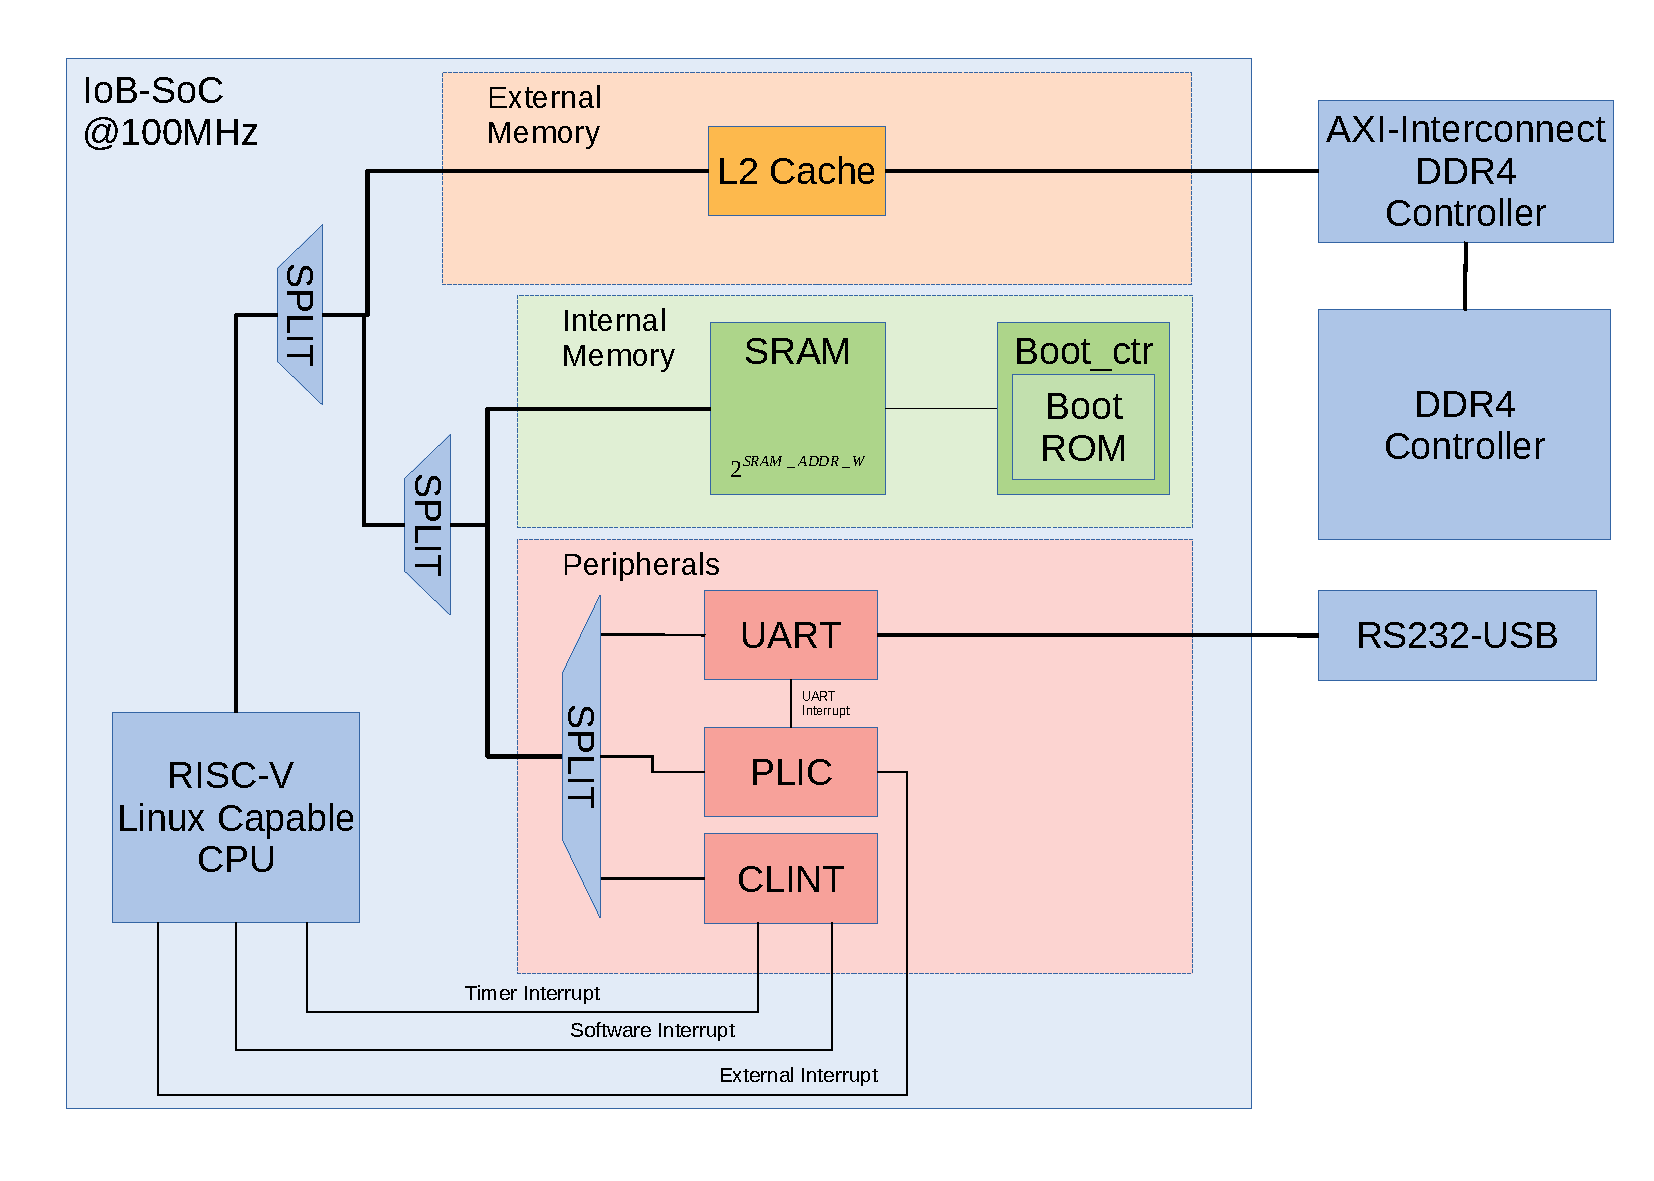
\includegraphics[width=0.7\linewidth]{bd_linux.pdf}
    \caption{Developed \acrshort{soc} sketch.}
    \label{fig:bd_linux}
\end{figure}

Comparing figure \ref{fig:bd_linux} with the original design of \textit{IOb-SoC} (figure \ref{fig:bd_original}) we can see that there were a few additional alterations. In the first place, it can be seen that the L1 Cache was removed. Since every application processor studied had an L1 cache built in, there was no need for the L1 \textit{iob-cache}. Next, a \textit{iob-split} was added to the \textit{IOb-SoC}. Previously, there was a single \textit{iob-split} for the data bus with three slaves (the internal memory, the external memory and the peripheral bus). This meant that there were 2 selection bits, when '00' then the internal memory bus was active, when '01' it was the peripheral bus and when '10' it was the external memory. This caused a problem because when addressing the external memory if its size is bigger than 1GB the selection bits would be '11'. The \acrfull{demux} output selected by '11' is not connected anywhere, so this caused an internal hardware error. The solution was to include two \textit{iob-split} modules each with two slaves. The first would choose between the external memory and either the internal memory or peripheral bus. The second would choose between the internal memory and the peripheral bus. Another advantage of using this method is that now the selection bit's position does not vary depending on if we are using the DDR or not. This makes it easier to use external software that does not use the \textit{iob-soc} Makefiles. Before the peripheral addressing on external software had to be changed every time the developer wanted to test with or without the external memory.

During this project, there was also an improvement on the \textit{IOb-SoC} verification. This led to the creation of a top hardware module for the developed \acrlong{soc}.

\section{Central Processing Unit}
\label{section:cpu}
The \acrshort{cpu} chosen to use in this project was \textit{VexRiscv}. The performance of the CPU is not a significant issue for this project. However, how the core was designed and developed highly influenced the CPU decision. The flexibility of the CPU design, meaning how easily the CPU can be adapted to take advantage of the other components in \textit{IOb-SoC}, is an essential factor. Since the hardware and software developed in this project are open-source, the CPU implemented had to be open-source hardware. Moreover, knowing that the \textit{IOb-SoC} signals are 32-bit wide, ideally, the selected CPU should support RV32IMAC to facilitate its integration with IOb-SoC. From the \acrshort{cpu}s studied in chapter \ref{chapter:existing_embedded_technologies} \textit{VexRiscv} looked like the more indicated.

Generating the \acrshort{rtl} \textit{verilog} file from the \textit{SpinalHDL} hardware description is very simple. After cloning the \textit{VexRiscv} GitHub repository the developer only has to run one command. As can be seen below in listing \ref{lst:rtl_vexriscv}. On the \textit{VexRiscv} repository there exist a couple of demo \acrshort{cpu} configurations. The configurations can be directly used or configured to generate a custom \textit{VexRiscv} core. There even already exists a demo configuration to generate a Linux-compatible core. Although in the developed hardware a custom core was implemented, the Linux demo configuration was used as a starting point. Unfortunately, the Linux Demo design is outdated and the instructions, commented on the hardware configuration file, to run a Linux simulation and test the core does not work.

\begin{lstlisting}[language=make, caption={Generate \textit{verilog} from \textit{SpinalHDL}}, label=lst:rtl_vexriscv]
git clone https://github.com/SpinalHDL/VexRiscv.git && \
  cd VexRiscv && sbt "runMain vexriscv.demo.LinuxGen"
\end{lstlisting}

The \textit{VexRiscv} can be configured by adding and removing plugins. Plugins are hardware components described in \textit{SpinalHDL} that can be reused in different designs by simply adding \enquote{\textcolor{green}{new} \textcolor{red}{Plugin\_Name}(...),} to the plugins list in the top \acrshort{cpu} description file. The existing plugins are described in the \textit{VexRiscv} repository on the \enquote{src/main/scala/vexriscv/plugin} directory. Looking at the available plugins it can be seen that there are two different plugins for the instruction bus and data bus. They are \enquote{IBusSimplePlugin}, \enquote{IBusCachedPlugin}, \enquote{DBusSimplePlugin} and \enquote{DBusCachedPlugin}. The difference is that the \enquote{cached} plugins have the L1 Cache integrated, while the simple plugins do not. An additional different between the data cached and simple plugin it that, although the \enquote{DBusCachedPlugin} fully supports the RISC-V atomic extension, the \enquote{DBusSimplePlugin} supports \acrfull{lr}/\acrfull{sc} but not \acrfull{amo} instructions. The \enquote{DBusSimplePlugin} could also be adapted to enable the full \enquote{A} extension, but since I do not understand how to code in \textit{SpinalHDL} it would be very time-consuming.

The first step on implementing the \textit{VexRiscv} core on the \textit{IOb-SoC} was making sure that it worked on \enquote{bare metal} applications. Meaning it had to be working with the application accessing the silicon chip directly without any intermediary like an \acrfull{os}. This was done using the instruction and data \enquote{simple} plugins. The next step was to run the Linux kernel. To do so the instruction and data \enquote{simple} plugins had to be changed to the \enquote{cached} plugins. The missing support for \acrfull{amo} instructions was noticeable because the software would stop executing and enable an unknown instruction signal. It was possible to identify which instruction was causing the problem through the signal waves created during simulation.

The final \textit{VexRiscv} core configuration file contained the needed plugins to run a minimal \acrfull{os} based on Linux. The plugins present were:
% The file can be found in the project git hub repository under (\url{https://github.com/IObundle/iob-vexriscv/blob/cached_vexriscv/software/vexriscv_core/Linux.scala}).
\begin{itemize}
  \item The \enquote{IBusCachedPlugin} was added. With it, the address of the first instruction the CPU had to fetch was defined by setting the reset value of the \acrfull{pc}. Also, it was specified that the CPU had no branch predictor and that it supported compressed instructions. The decision to not use any branch predictor was because there seemed to be a compatibility problem between the most recent RISC-V toolchain and the branch predictor that are available in the \textit{VexRiscv}. Since performance was not a concern in this project I choose to not use a branch predictor.
  \item The \enquote{DBusCachedPlugin} was added for the reason that it fully supported the atomic instructions.
  \item The \enquote{DecoderSimplePlugin} is used to decode the instructions.
  \item The \enquote{RegFilePlugin} implements the register file. These are the registers inside the CPU.
  \item The \enquote{IntAluPlugin} is used to calculate arithmetic and logic operations.
  \item The \enquote{SrcPlugin} is an auxiliary plugin for the plugins that contain \acrfull{alu}, Branch related hardware and Load/Store hardware logic.
  \item The \enquote{FullBarrelShifterPlugin} implements the shift instructions present in the RISC-V base \acrfull{isa}.
  \item The \enquote{HazardSimplePlugin} is used by the core to determine where it needs to stall.
  \item The \enquote{MulPlugin} allows the core to execute multiplication instructions.
  \item The \enquote{MulDivIterativePlugin} could be used to add multiplication and division support to the core (RISC-V M \acrshort{isa} extension). In this case, it was used to add only division since the multiplication support was added by another plugin.
  \item The \enquote{CsrPlugin} is configured to fully support Linux. This plugins adds the needed \acrfull{csr} to run a full feature \acrshort{os}.
  \item The \enquote{DebugPlugin} was deactivated in the used core. But it could be used to debug the CPU core if there existed a JTAG interface. Currently the \textit{IOb-SoC} does not support it.
  \item The \enquote{BranchPlugin} allows the core to execute and make decisions on the jump instructions. This is part of the base \acrfull{isa}
  \item The \enquote{MmuPlugin} added support for the \acrfull{mmu}. Which is required to run a full feature \acrshort{os}.
  \item The \enquote{FpuPlugin} can add support for both the floats and doubles instruction extensions. In the core used this plugin was deactivated since to run a minimal \acrshort{os} there is little to no advantage of using this extension. Causing the FPU to only be adding unnecessary hardware logic.
  %\item The \enquote{YamlPlugin} offers a service to other plugins to generate a useful Yaml file describing the CPU configuration. % It needs to be there for some reason. I am dunno.
\end{itemize}

After generating the Verilog file that describes a \textit{VexRiscv} core I had to create a wrapper hardware module that adapted the \textit{VexRiscv} core interface to the \textit{IOb-SoC} internal bus.

\subsection{VexRiscv Wrapper}
The Verilog wrapper, witch is called \textit{iob\_VexRiscv}, is instantiated by the \textit{IOb-SoC} top \acrshort{soc} hardware module as the \acrshort{cpu} component and instantiates the \textit{VexRiscv} core Verilog module. The interface between the \textit{IOb-SoC} hardware and the \textit{VexRiscv} core is created by establishing a connection between the inputs and outputs from both sides.

The input signals of \textit{iob\_vexriscv} are the clock signal which is the system clock derivative from the development board where the \acrshort{soc} is implemented; the reset signal which is set to high ('1') when the system reboots and when the stage 0 bootloader finishes; the boot signal that has the value '1' while the stage 0 bootloader is executing, after it finishes the boot signal value drops to '0' at the same time the reset signal is set to high; the instruction bus response signal that is connected to \enquote{cpu\_i\_resp}; the data bus response signal that is connected to \enquote{cpu\_d\_resp}; the timer interrupt and software interrupt signals which are set to '1' or '0' by the \acrshort{clint} unit; the external interrupt signal which is controlled by the \acrshort{plic} unit. The output signals are the instruction bus request signal and the data bus request signal, which connect to the \enquote{cpu\_i\_req} and \enquote{cpu\_d\_req} respectably. The \enquote{cpu\_i\_resp}, \enquote{cpu\_d\_resp}, \enquote{cpu\_i\_req} and \enquote{cpu\_d\_req} signals were reviewed in section \ref{section:the_iob_soc_template}.

The input and output signals of the \textit{VexRiscv} core can be seen in table \ref{tab:vexriscv_core_and_iob_soc}. It can also be seen the signal's width and their equivalent signal in the \textit{IOb-SoC} top hardware.

\begin{table}[!ht]
  \centering
  \resizebox{\textwidth}{!}{%
  \begin{tabular}{|l|l|l|l|l|}
    \hline
    \textbf{Port}                & \textbf{Width} & \textbf{Direction} & \textbf{Description}                                                                                          & \textbf{IOb-SoC Port}           \\ \hline
    dBus\_cmd\_valid             & 1              & output             & \begin{tabular}[c]{@{}l@{}}Indicates that the CPU is ready\\  to make a data request.\end{tabular}            & cpu\_d\_req{[}`valid(0){]}      \\ \hline
    dBus\_cmd\_ready             & 1              & input              & \begin{tabular}[c]{@{}l@{}}Indicates that the SoC is ready\\  to receive a data request.\end{tabular}         & N/A                             \\ \hline
    dBus\_cmd\_payload\_wr       & 1              & output             & \begin{tabular}[c]{@{}l@{}}Indicates that the CPU wants\\  to write data to memory.\end{tabular}              & N/A                             \\ \hline
    dBus\_cmd\_payload\_uncached & 1              & output             & Indicates if data is on L1 cache                                                                              & Not used                        \\ \hline
    dBus\_cmd\_payload\_address  & 32             & output             & Used to address memory.                                                                                       & cpu\_d\_req{[}`address(0,32){]} \\ \hline
    dBus\_cmd\_payload\_data     & 32             & output             & Used to send data to memory.                                                                                  & cpu\_d\_req{[}`wdata(0){]}      \\ \hline
    dBus\_cmd\_payload\_mask     & 4              & output             & \begin{tabular}[c]{@{}l@{}}Indicates which bytes in a\\  word are accessed.\end{tabular}                      & N/A                             \\ \hline
    dBus\_cmd\_payload\_size     & 2              & output             & $log_2$(number of bytes in the burst)                                                                         & Not used                        \\ \hline
    dBus\_cmd\_payload\_last     & 1              & output             & \begin{tabular}[c]{@{}l@{}}Indicates when the last\\  byte is transferred.\end{tabular}                       & Not used                        \\ \hline
    dBus\_rsp\_valid             & 1              & input              & \begin{tabular}[c]{@{}l@{}}Indicates that the SoC is ready\\  to send a response.\end{tabular}                & cpu\_d\_resp{[}`valid(0){]}     \\ \hline
    dBus\_rsp\_payload\_last     & 1              & input              & \begin{tabular}[c]{@{}l@{}}Indicates when the last\\  byte is transferred.\end{tabular}                       & Not used                        \\ \hline
    dBus\_rsp\_payload\_data     & 32             & input              & Receive data from memory.                                                                                     & cpu\_d\_resp{[}`rdata(0){]}     \\ \hline
    dBus\_rsp\_payload\_error    & 1              & input              & Indicates existence of an error.                                                                              & Not used                        \\ \hline
    timerInterrupt               & 1              & input              & Indicate a Timer Interrupt.                                                                                   & timerInterrupt                  \\ \hline
    externalInterrupt            & 1              & input              & Indicate an External Interrupt.                                                                               & externalInterrupt               \\ \hline
    softwareInterrupt            & 1              & input              & Indicate a Software Interrupt.                                                                                & softwareInterrupt               \\ \hline
    externalInterruptS           & 1              & input              & \begin{tabular}[c]{@{}l@{}}Indicate an External Interrupt\\  at the Supervisor level.\end{tabular}            & Not used                        \\ \hline
    iBus\_cmd\_valid             & 1              & output             & \begin{tabular}[c]{@{}l@{}}Indicates that the CPU is ready\\  to make an instruction request.\end{tabular}    & cpu\_i\_req{[}`valid(0){]}      \\ \hline
    iBus\_cmd\_ready             & 1              & input              & \begin{tabular}[c]{@{}l@{}}Indicates that the SoC is ready\\  to receive an instruction request.\end{tabular} & N/A                             \\ \hline
    iBus\_cmd\_payload\_address  & 32             & output             & Used to address memory.                                                                                       & cpu\_i\_req{[}`address(0,32){]} \\ \hline
    iBus\_cmd\_payload\_size     & 2              & output             & $log_2$(number of bytes in the burst)                                                                         & Not used                        \\ \hline
    iBus\_rsp\_valid             & 1              & input              & \begin{tabular}[c]{@{}l@{}}Indicates that the SoC is ready\\  to send a response.\end{tabular}                & cpu\_i\_resp{[}`valid(0){]}     \\ \hline
    iBus\_rsp\_payload\_data     & 32             & input              & Receive an instruction from memory.                                                                           & cpu\_i\_resp{[}`rdata(0){]}     \\ \hline
    iBus\_rsp\_payload\_error    & 1              & input              & Indicates existence of an error.                                                                              & Not used                        \\ \hline
    clk                          & 1              & input              & System clock signal.                                                                                          & clk                             \\ \hline
    reset                        & 1              & input              & CPU reset signal.                                                                                             & cpu\_reset                      \\ \hline
    \end{tabular}%
  }
  \caption{\textit{VexRiscv} core inputs and outputs.}
  \label{tab:vexriscv_core_and_iob_soc}
\end{table}

After understanding the inputs and outputs of each module it is easy to see which wires should be connected. But after connecting all the wires there were three problems. The first was the \enquote{strb} signal needed by \textit{IOb-SoC} when writing data to memory which did not exist in the \textit{VexRiscv} signals. The \enquote{strb} signal could be obtained in two different ways. One way would be through the \enquote{dbus\_req\_size} signal, the two less significant bits of the \enquote{dbus\_req\_address} and the \enquote{dbus\_req\_wr} signal. The other way was through the \enquote{dBus\_cmd\_payload\_mask} signal and the \enquote{dBus\_cmd\_payload\_wr} signal. The \enquote{DBusSimplePlugin}, contrary to the \enquote{DBusCachedPlugin}, had no \enquote{dBus\_cmd\_payload\_mask} signal that is why the first method was created. Accordingly for the first method, the \enquote{mask} signal had to be generated by the hardware logic expressed in equation \ref{eq:mask_generated}. % Should I make a figure with a MUX and a shifter?

\begin{equation}
  \begin{cases}
    dbus\_req\_mask\_aux = dbus\_req\_size[1] ? {4'hF} : (dbus\_req\_size[0] ? {4'h3} : {4'h1}) \\
    dbus\_req\_mask = dbus\_req\_mask\_aux << dbus\_req\_address[1:0]
  \end{cases}
  \label{eq:mask_generated}
\end{equation}

Moreover, the \enquote{mask} signal indicated the active bytes when both read or write operations were occurring. On the other hand, the \enquote{strb} signal should only be active when a write operation is happening. Both methods logic expressions can be seen in equation \ref{eq:strb_vexriscv}. This implements a \acrshort{mux} where \enquote{dbus\_req\_wr} is the selection bit.

\begin{equation}
  \begin{split}
  strb& = dbus\_req\_wr ? dbus\_req\_mask : 4'h0 \\
      & = dbus\_req\_wr ? dBus\_cmd\_payload\_mask : 4'h0
  \end{split}
  \label{eq:strb_vexriscv}
\end{equation}

The second is that the \textit{IOb-SoC} internal bus did not contain all the signals that were needed by the \textit{VexRiscv} core. To successfully make the interface handshake with the \textit{VexRiscv} core an instruction and data request \enquote{ready} signal had to be generated. The \enquote{ready} signal indicated that the \acrshort{soc} was ready to receive and accept a request from the CPU. To solve this problem a register that saved the value of the \enquote{cmd\_valid}, called \enquote{valid\_reg}, was created. This register would be updated when either the \enquote{cmd\_valid} or the \enquote{rsp\_valid} signal were active. The \enquote{ready} signal should be high ('1') before accepting a request, and after it should be low ('0') while the response is not available. The initial approach to the values that the \enquote{cmd\_ready} signal should assume can be seen in the truth table \ref{tab:first_truth_table}. This truth table was obtained by analyzing the simulation signals wave. The \enquote{N/A} values in the table mean that those situations never occurred.

\begin{table}[!h]
  \centering
  \begin{tabular}{ccc|c}
  valid\_reg & cmd\_valid & rsp\_valid & cmd\_ready \\ \hline
  0          & 0          & 0          & 0          \\
  0          & 0          & 1          & N/A        \\
  0          & 1          & 0          & 1          \\
  0          & 1          & 1          & N/A        \\
  1          & 0          & 0          & 0          \\
  1          & 0          & 1          & 1          \\
  1          & 1          & 0          & 0          \\
  1          & 1          & 1          & 1         
  \end{tabular}
  \caption{First try at identifying the rules the cmd\_ready should follow.}
  \label{tab:first_truth_table}
\end{table}

The truth table can be transformed in a logic gates expression, which can be seen in equation \ref{eq:first_logic_eq}.

\begin{equation}
  (valid\_reg \cdot rsp\_valid) + (valid \cdot \overline{valid\_reg} \cdot \overline{rsp\_valid})
  \label{eq:first_logic_eq}
\end{equation}

But this approach had an issue. The logic expression depended on the \enquote{cmd\_valid} signal which was generated inside the \textit{VexRiscv} core. This could generate a bigger complication since the combinatorial circuit that generates the \enquote{cmd\_valid} is unknown and might generate an infinite hardware loop. From better analyzing the signal behavior it was noticed that when \enquote{valid\_reg}, \enquote{cmd\_valid} and \enquote{rsp\_valid} are low ('0') the value of \enquote{cmd\_ready} is irrelevant. It could be concluded since when the \enquote{valid\_reg}, \enquote{cmd\_valid} and \enquote{rsp\_valid} are low happens the \enquote{cmd\_ready} signal was not being used by the \textit{IOb-SoC}. The truth table can them be simplified to table \ref{tab:simple_truth_table}.

\begin{table}[!ht]
  \centering
  \begin{tabular}{cc|c}
  valid\_reg & rsp\_valid & req\_ready \\ \hline
  0          & 0          & 1          \\
  0          & 1          & N/A        \\
  1          & 0          & 0          \\
  1          & 1          & 1         
  \end{tabular}
  \caption{Simplified truth table.}
  \label{tab:simple_truth_table}
\end{table}

Which can be seen as a simple XOR logic gate. The equation \ref{eq:simple_logic_eq} show the hardware logic expression implement.

\begin{equation}
  (valid_reg \cdot rsp\_valid) + (\overline{valid_reg} \cdot \overline{rsp\_valid}) = valid_reg \odot rsp\_valid
  \label{eq:simple_logic_eq}
\end{equation}

The last problem was that after accepting an instruction or data request the values of the \enquote{address}, \enquote{data} and \enquote{mask} signals could change inside the \textit{VexRiscv} core. This changes would pass through \textit{iob\_VexRiscv} and reflect in the rest of \textit{IOb-SoC} hardware. Which caused the \textit{iob-cache} and peripherals to not function currently. This problem was solved by creating registers that saved the value of the \enquote{address}, \enquote{data} and \enquote{strb} signals when the request was accepted. The register values would then only change when the response was already received.

To finalize, the \acrshort{cpu} should be able to run firmware from both the internal and external memory. When the stage 0 bootloader is running the \acrfull{msb} of the instruction fetched address had to be forced to '0'. This would force the \acrshort{cpu} to fetch instructions from the boot hardware unit. When defined that the firmware had to run from the external memory (RUN\_EXTMEM=1) the first instruction fetched should be at address $0x80000000$. To achieve this requirement the \acrfull{msb}, when RUN\_EXTMEM=1 was defined as the negated value of the boot signal. When RUN\_EXTMEM=0 the \acrshort{msb} was forced to always be '0' since there is no need to access the external memory. On the data request bus, it should also be taken into account that the \acrshort{msb} had to be '0' when the \acrshort{cpu} wanted to access the peripherals.

\section{\textit{UART 16550}}
\label{section:uart}
The approach taken in this project was to adapt an existing open-source \acrfull{uart} core that is supported by the Linux kernel. The other option was to create a Linux driver compatible with \textit{iob-UART} and compile the kernel with it. The chosen approach seemed more adequate and a simpler solution.

Since the developed chip is supposed to be open-source the \acrshort{uart} core should also be open-source hardware. The core used was a \textit{\acrshort{uart}16550}~\cite{gorban2002uart} that has been made available by \textit{freecores} on \textit{github}. This \acrshort{uart} was written in Verilog, although it was an older version of Verilog it is still synthesisable by modern tools and easy to understand. The \textit{UART16550} core used implements a wishbone interface to interact with the \acrfull{soc}. Similarly to what was done with the CPU, I had to create a wrapper to adapt the core to the \textit{IOb-SoC}.

\subsection{\textit{UART 16550} Wrapper}
The wishbone interface is established in the top hardware module from the used \textit{UART16550} core. In table \ref{tab:uart16550_wishbone}, which can be obtained from the open-source \textit{UART16550} core documentation, it can be seen the wishbone interface signals. The wishbone specification determines that there needs to be a master and a slave. In this case when the \acrshort{cpu} sends a request signal for the \textit{UART16550} peripheral the master is the \acrshort{cpu} and the slave is the \textit{UART16550}.

\begin{table}[!ht]
  \centering
  \begin{tabular}{|l|l|l|l|}
  \hline
  \textbf{Port} & \textbf{Width} & \textbf{Direction} & \textbf{Description}          \\ \hline
  CLK           & 1              & Input              & Block's clock input           \\ \hline
  WB\_RST\_I    & 1              & Input              & Asynchronous Reset            \\ \hline
  WB\_ADDR\_I   & 5 or 3         & Input              & Used for register selection   \\ \hline
  WB\_SEL\_I    & 4              & Input              & Select signal                 \\ \hline
  WB\_DAT\_I    & 32 or 8        & Input              & Data input                    \\ \hline
  WB\_DAT\_O    & 32 or 8        & Output             & Data output                   \\ \hline
  WB\_WE\_I     & 1              & Input              & Write or read cycle selection \\ \hline
  WB\_STB\_I    & 1              & Input              & Specifies transfer cycle      \\ \hline
  WB\_CYC\_I    & 1              & Input              & A bus cycle is in progress    \\ \hline
  WB\_ACK\_O    & 1              & Output             & Acknowledge of a transfer     \\ \hline
  \end{tabular}
  \caption{WISHBONE interface signals.}
  \label{tab:uart16550_wishbone}
\end{table}

The interface between the \textit{IOb-SoC} and the \textit{UART16550} top hardware is established by the verilog module that acts as a \textit{UART16550} wrapper. The wrapper module is called \enquote{iob\_uart16550}. The \enquote{iob\_uart16550} hardware component has to generate the missing signal that are needed by the wishbone interface but do not exist in \textit{IOb-SoC}. In table \ref{tab:wishbone_iob_soc} the connection between the \textit{IOb-SoC} and the \textit{UART16550} wishbone interface can be analyzed. The missing signal are the \enquote{WB\_SEL\_I}, the \enquote{WB\_WE\_I} and the \enquote{WB\_STB\_I}. The select signal is similar to the \enquote{strb} signal but it should exist during write and read operations. This signal can be obtained through the two \acrfull{lsb} of the address signal. And since registers are addressed byte by byte only one bit at a time will be set to high on the select signal. The write signal is set to high whenever the \acrshort{cpu} wants to write to the \textit{UART16550} registers. This can be perceived through the \textit{IOb-SoC} \enquote{strb} signal. If any of the \enquote{strb} bits are enabled the \enquote{WB\_WE\_I} signal should be high ('1'). The transfer cycle should happen (i.e. \enquote{WB\_STB\_I} signal should be set to '1') when the \textit{UART16550} has accepted a request but still has not issued the response. Furthermore, the \textit{UART16550} has an interrupt output pin that is connected to the \acrshort{soc} \enquote{uartInterrupt}. The \acrshort{soc} \enquote{uartInterrupt} is then passed to the \acrshort{plic} unit.

\begin{table}[!ht]
  \centering
  \resizebox{\textwidth}{!}{%
  \begin{tabular}{|l|l|l|}
  \hline
  \textbf{UART16550 Wishbone} & \textbf{IOb-UART16550}                  & \textbf{IOb-SoC}                         \\ \hline
  CLK                         & clk                                     & clk                                      \\ \hline
  WB\_RST\_I                  & rst                                     & reset                                    \\ \hline
  WB\_ADDR\_I                 & address{[}`UART\_ADDR\_WIDTH-1:0{]}     & slaves\_req{[}`address(`UART16550,32){]} \\ \hline
  WB\_SEL\_I                  & 1\textless{}\textless{}address{[}1:0{]} & N/A                                      \\ \hline
  WB\_DAT\_I                  & wdata                                   & slaves\_req{[}`wdata(`UART16550){]}      \\ \hline
  WB\_DAT\_O                  & rdata                                   & slaves\_resp{[}`rdata(`UART16550){]}     \\ \hline
  WB\_WE\_I                   & | wstrb                                 & N/A                                      \\ \hline
  WB\_STB\_I                  & valid\&($\sim$ready)                    & N/A                                      \\ \hline
  WB\_CYC\_I                  & valid                                   & slaves\_req{[}`valid(`UART16550){]}      \\ \hline
  WB\_ACK\_O                  & ready                                   & slaves\_resp{[}`ready(`UART16550){]}     \\ \hline
  \end{tabular}%
  }
  \caption{\textit{UART16550} interface with \textit{IOb-SoC}.}
  \label{tab:wishbone_iob_soc}
\end{table}

Finally, the \enquote{iob\_uart16550} also has to pass the interface between the \textit{UART16550} core and the RS232 connector. That is why it implements the: txd output to transmit data through serial; the rxd input to receive data through serial; the cts input which indicates that the destination is ready to receive a transmission sent by the UART; the rts output which indicates that the UART is ready to receive a transmission from the sender. Those pins are connected to the development board RS232 connector.

\section{CLINT Unit}
\label{section:clint}
The \acrshort{clint} was the only hardware component that was developed from scratch. Even though, there already exist open-source \acrfull{clint} hardware modules. For example, the \acrshort{clint} used with the \textit{CVA6} core and developed by the \textit{PULP platform}. The problem with this \acrshort{clint} module is that it is written in system-Verilog and uses packages and definitions from the \textit{CVA6} core. The \acrshort{clint} core is a simple hardware component. Considering that it only needs a few registers and signals to work, as it was studied in section \ref{section:riscv}. The interface with \textit{IOb-SoC} would have to be developed independently of the \acrshort{clint} core used. The best solution was to fully create the \acrshort{clint} hardware unit.

The inputs and outputs of the \acrshort{clint} unit can be seen in table \ref{tab:clint_signals}. \enquote{N\_CORES} is the number of \acrshort{cpu} core that are used in the \acrshort{soc}. In the \acrfull{soc} developed there is only one core. But the \acrshort{clint} is built with a multi-core system in mind. Each core has its timer and software interrupt. As such, the \enquote{mtip} and \enquote{msip} registers width is the number of core, \enquote{N\_CORES}.

\begin{table}[!ht]
  \centering
  \resizebox{\textwidth}{!}{%
  \begin{tabular}{|l|l|l|l|l|}
  \hline
  \textbf{Port} & \textbf{Width} & \textbf{Direction} & \textbf{Description}                                                                                & \textbf{IOb-SoC Port}                \\ \hline
  clk           & 1              & input              & System clock                                                                                        & clk                                  \\ \hline
  rst           & 1              & input              & System reset                                                                                        & reset                                \\ \hline
  rt\_clk       & 1              & input              & Real-time clock                                                                                     & rtc                                  \\ \hline
  valid         & 1              & input              & \begin{tabular}[c]{@{}l@{}}Indicates that the CPU is ready\\   to make a data request.\end{tabular} & slaves\_req{[}`valid(`CLINT){]}      \\ \hline
  address       & 32             & input              & Register address.                                                                                   & slaves\_req{[}`address(`CLINT,16){]} \\ \hline
  wdata         & 32             & input              & Data to write to register.                                                                          & slaves\_req{[}`wdata(`CLINT){]}      \\ \hline
  wstrb         & 4              & input              & Used to generate a "write" signal.                                                                  & slaves\_req{[}`wstrb(`CLINT){]}      \\ \hline
  rdata         & 32             & output             & Data read from register.                                                                            & slaves\_resp{[}`rdata(`CLINT){]}     \\ \hline
  ready         & 1              & output             & \begin{tabular}[c]{@{}l@{}}Indicates that the CLINT is ready\\   to send a response.\end{tabular}   & slaves\_resp{[}`ready(`CLINT){]}     \\ \hline
  mtip          & N\_CORES       & output             & Raise a timer interrupt in a core.                                                                  & timerInterrupt                       \\ \hline
  msip          & N\_CORES       & output             & Raise a software interrupt in a core.                                                               & softwareInterrupt                    \\ \hline
  \end{tabular}%
  }
  \caption{CLINT interface with \textit{IOb-SoC}.}
  \label{tab:clint_signals}
\end{table}

The \enquote{rt\_clk} signal, although it is connected to \enquote{rtc} wire, is not available in \textit{IOb-SoC} since the development board does not have any \acrfull{rtc} crystal connected. The \acrshort{rtc} frequency is commonly 32.768 kHz, because it is a power of 2 ($2^15$) value. To get a precise 1-second period (1 Hz frequency) would only be needed a 15 stage binary counter. With a \acrshort{rtc} the \acrshort{clint} unit had to detect the rising edge of the \enquote{rt\_clk} signal. The rising edge was detected by taking samples of the \enquote{rt\_clk} signal at the system clock frequency. This is possible because the \acrshort{rtc} is slower than the system clock. If in the future the \acrshort{clint} unit developed is implemented in a system with a \acrshort{rtc} the hardware design can be easily adapted to it. Since the logic was already developed. % Talk about meta stability??

In the development boards used there is no \acrshort{rtc} so an alternative had to be found. The method implemented was simpler than the logic if there existed a \acrshort{rtc}. The system clock operates at 100 MHz so a counter was added to the design and each time that counter reached 999 the timer register would increment. Like this, a \acrshort{rtc} working at 100 kHz was simulated in the \acrshort{clint} hardware.

Concluding, the needed registers to develop a \acrshort{clint} unit in accordance with the RISC-V specifications were implemented. And the hardware logic needed to trigger the timer and software interrupts were described.

\section{PLIC Unit}
\label{section:plic}
The \acrshort{plic} is not essential to run a full feature \acrfull{os} on a \acrfull{soc}. Since the \acrshort{plic} is used to drive interrupts generated by other peripherals to the core, in this project the only peripheral connected to the \acrshort{plic} is the \textit{UART16550}. For the growth of the \acrshort{soc}, the \acrshort{plic} unit is very useful and a requirement to have. Some peripherals that might be added in the future also use the \acrshort{plic} hardware, for example, the \textit{ethernet} controller can be used to wake a core from low power mode.

Since the \acrshort{plic} hardware unit is more complex then the \acrshort{clint}, it was decided that an open-source \acrshort{plic} core would be adapted for the \textit{IOb-SoC}. There were three available cores. The \acrshort{plic} developed by \textit{lowRISC}~\cite{lowrisc_plic} is written in a variation of \textit{System Verilog}, consequently it is difficult to adapt and test. The \acrshort{plic} used with the \textit{CVA6} core, developed by the \textit{PULP platform}~\cite{pulp_plic}, started as a fork of an older version of the \textit{lowRISC}. This \acrshort{plic} unit is written in pure \textit{System Verilog}. I tried to adapt the \acrshort{plic} unit from \textit{PULP platform} but there were many incompatibilities with the \textit{IOb-SoC}. Finally, the \acrshort{plic} developed by \textit{RoaLogic}~\cite{roalogic_plic} was the hardware unit used as a starting point. The \textit{RoaLogic} \acrshort{plic} is also written in \textit{System Verilog} and implements an \textit{apb4} or \textit{ahb3lite} interface with the \acrshort{soc}. The biggest advantage of the \textit{RoaLogic} hardware is that the \acrshort{plic} relevant components for the \textit{IOb-SoC}, the \acrshort{plic} registers and core, are well separated from the modules that create the interface with the \acrshort{soc} and instantiate them. To integrate the a \acrshort{plic} unit on the \textit{IOb-SoC} I had to develop a \acrshort{plic} wrapper.

\subsection{PLIC wrapper}
The \acrshort{plic} wrapper had to create the interface with the \textit{IOb-SoC} internal buses. Furthermore, it needed to instantiate the \acrshort{plic} registers and core hardware modules.
....

\section{UUT Top Hardware}
\label{section:uut}
This top module creates a \textit{verilog} wrapper of the \acrfull{uut} that allows it to interact with the different hardware logic simulators. The top module file is an adaptation of the previous \textit{verilog} file used on the Icarus simulation.

\begin{figure}[!ht]
    \centering
    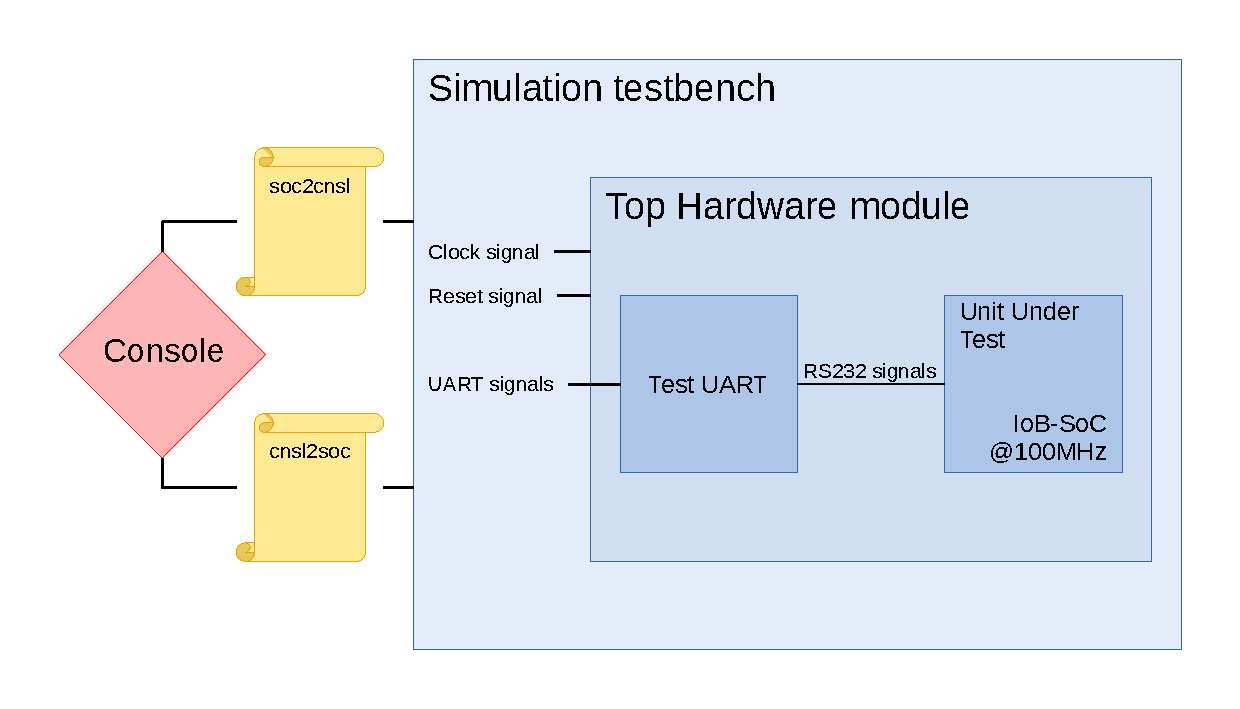
\includegraphics[width=\linewidth]{uut_top_hw.pdf}
    \caption{Simulated hardware interfaces.}
    \label{fig:uut_top_hw}
\end{figure}

\chapter{Software Developed}

\section{Python Console}

\section{Verilator Testbench}
\subsection{UUT Top Hardware module}
\label{section:uut}
This top module creates a \textit{verilog} wrapper of the \acrfull{uut} that allows it to interact with the different hardware logic simulators. Even tho this is written harddware logic it is never implemented as real hardware. This module is only used in simulation as software.

The top module file is an adaptation of the previous \textit{verilog} file used on the Icarus simulation. Previously, the verilog top file would interact directly with the console. Similarly to the new hardware top module an \acrshort{uart} module is instantiated and a serial connection with the \textit{IOb-SoC} is simulated. Although in this project the \textit{IOb-UART} in the \acrfull{soc} was swapped for the \textit{UART16550} in the 

\begin{figure}[!ht]
    \centering
    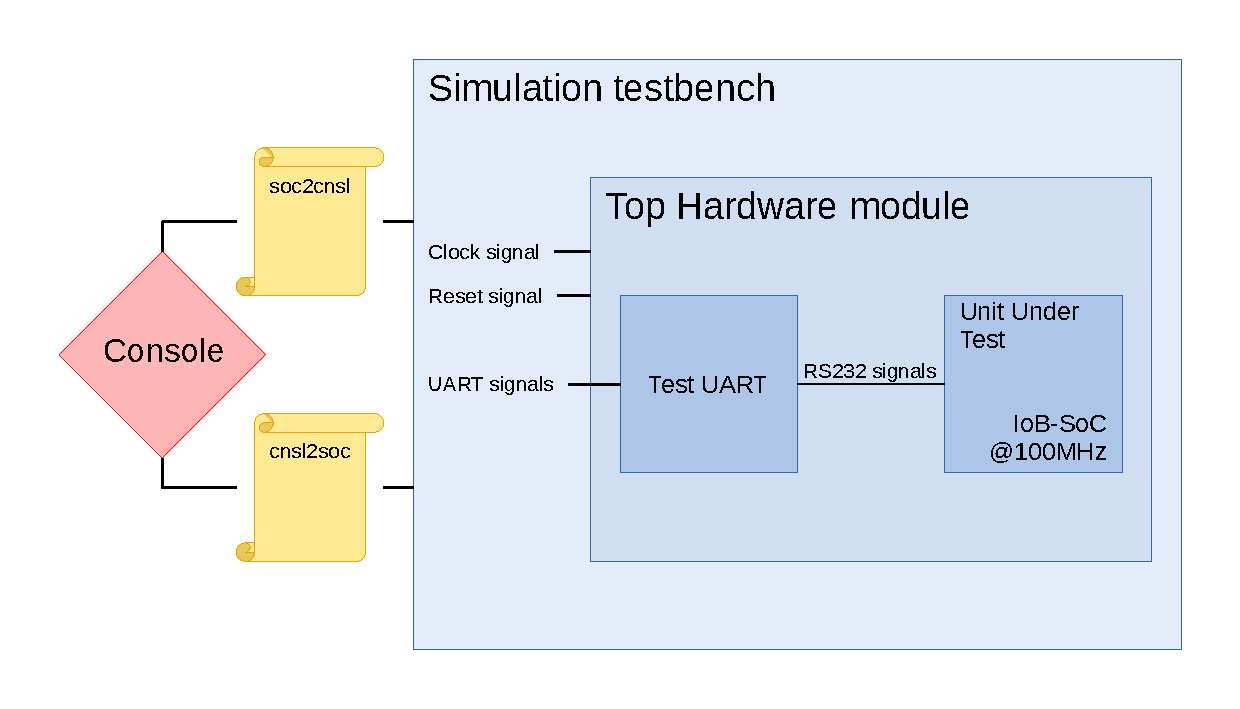
\includegraphics[width=\linewidth]{uut_top_hw.pdf}
    \caption{Simulated hardware interfaces.}
    \label{fig:uut_top_hw}
\end{figure}

\section{Barebones Interrupt Routine}

\section{IOb-SoC Linux Stage 0 Bootloader}

\section{IOb-SoC on OpenSBI}

\section{IOb-SoC Device Tree}

\section{IOb-SoC Linux \textit{'rootfs'}}

\section{Makefiles}
\chapter{Project Results}
\label{chapter:project_results}
In the following chapter, the author will analyse the results obtained from the hardware and software developed in this thesis project. The author's first objective was running the \enquote{Hello World!} firmware with the \textit{VexRiscv} \acrshort{cpu}. Secondly, he tested the implementation of the interrupt routine software with the developed \acrshort{clint} hardware. Finally, the candidate successfully executed the minimal Linux \acrshort{os} in real hardware using the developed \acrlong{soc}.

All the results obtained in this thesis which communicate with the \acrshort{fpga} board or the \acrshort{soc} testbench, are executing the developed \textit{Console} program. The hardware components comprising the \acrshort{soc} differ in each section of this chapter. The author customises the \acrshort{soc} hardware depending on the software needs.

In each step, the author studied the simulation with the different logic simulators and the memory resources needed to run the respective firmware. Furthermore, when running the \acrshort{soc} on the \acrshort{fpga} board he examined the required \acrshort{fpga} resources.

\section{System Running \enquote{Hello World!}}
\label{section:hello_world}
The \textit{IObundle} developers created the \enquote{Hello World!} firmware to test the functionality of the \textit{IOb-SoC} template. After the author implemented the \textit{VexRiscv} \acrshort{cpu} on the developed \acrshort{soc}, he executed a regression test to verify the correctness of the \acrshort{soc}. The regression test was the execution of the \enquote{Hello World!}, which was known to work correctly on the \textit{IOb-SoC}.

The \enquote{Hello World!} firmware is a program that prints a \enquote{Hello World!} message to the user, prints the value of $\pi$, which is a floating number, and tests file transferring between the \textit{Console} and \textit{IOb-SoC}. The only alteration the author made to the \textit{IOb-SoC} hardware to obtain the results presented in this section was swapping the \acrshort{cpu}.

The \enquote{Hello World!} program size is 23964 Bytes. The minimal size of the memory on the \acrshort{soc} is dictated by the firmware size. The memory size should be the closest upper bound power of two.

\subsection{Execute in simulation}
The author simulated the \enquote{Hello World!} program using the \textit{Icarus} simulator and \textit{Verilator}. The \enquote{Hello World!} simulation allows the author to make a fair comparison between both logic simulators.

In figure \ref{fig:hello_sim} the reader can see the expected output when executing the \enquote{Hello World!} firmware. In this example, the simulator executed the firmware using the internal memory of the \acrshort{soc} and considered that the firmware was already on the memory. Considering the firmware was already on the memory, allow the simulator not to execute the firmware transfer between the \textit{Console} and the testbench.

\begin{figure}[!ht]
    \centering
    \begin{subfigure}[b]{0.49\textwidth}
        \centering
        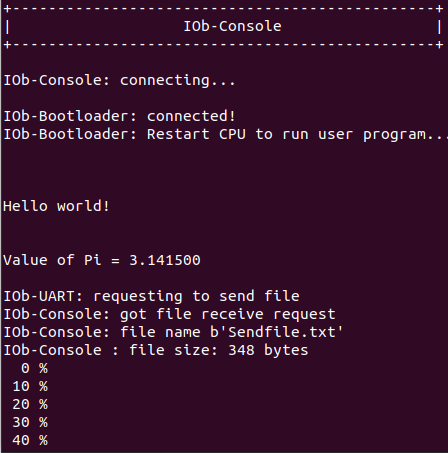
\includegraphics[width=\textwidth]{start_Hello_sim.png}
        \caption{Start of the \enquote{Hello World!} firmware.}
        \label{fig:start_hello_sim}
    \end{subfigure}
    \hfill
    \begin{subfigure}[b]{0.49\textwidth}
        \centering
        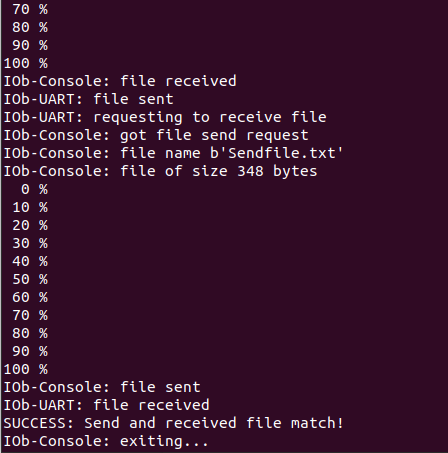
\includegraphics[width=\textwidth]{end_Hello_sim.png}
        \caption{End of the \enquote{Hello World!} firmware.}
        \label{fig:end_hello_sim}
    \end{subfigure}
    \caption{Running the \enquote{Hello World!} firmware in simulation.}
    \label{fig:hello_sim}
\end{figure}

Both open-source logic simulators are capable of executing the \enquote{Hello World!} program. When the baud rate decreases or the memory size increases the simulation is slower. The baud rate used in the simulation was 5000000, which is the number of bits per second transferred to the \acrshort{uart}. The simulations were run considering the system clock frequency 100MHz. The bootloader is always stored in internal memory. The bootloader memory is 4KB ($2^12$), since the bootloader binary is 1508 Bytes 4KB is enough memory to store the bootloader program. The firmware by default is stored in the internal memory and the memory size is 32KB ($2^15$). In table \ref{tab:hello_sim} the reader can see a timing comparison between the different logic simulators simulating the original \textit{IOb-SoC} and the developed \acrshort{soc}. The \enquote{INIT\_MEM} flag indicates whether the firmware is already loaded in the \acrshort{fpga} or if the \textit{Console} needs to transfer the firmware to the \acrshort{soc}, the user can set the flag to '1' or '0' respectively. The simulations can be executed with or without external memory. Furthermore, the firmware can run in the internal or external memory. The \enquote{make sim-test} command tests the different possible simulations.

\begin{table}[!ht]
    \centering
    \begin{tabular}{l|ll|ll|}
    \cline{2-5}
                                                           & \multicolumn{2}{l|}{Authors \acrshort{soc}} & \multicolumn{2}{l|}{\textit{IOb-SoC}}    \\ \hline
    \multicolumn{1}{|l|}{Command \textbackslash Simulator} & \multicolumn{1}{l|}{Icarus}  & Verilator & \multicolumn{1}{l|}{Icarus}  & Verilator \\ \hline
    \multicolumn{1}{|l|}{make sim-run INIT\_MEM=1}              & \multicolumn{1}{l|}{2m 26s}  & 0m 3s     & \multicolumn{1}{l|}{0m 25s}  & 0m 3s     \\ \hline
    \multicolumn{1}{|l|}{make sim-run INIT\_MEM=0}              & \multicolumn{1}{l|}{88m 19s} & 1m 1s     & \multicolumn{1}{l|}{15m 18s} & 0m 27s    \\ \hline
    \multicolumn{1}{|l|}{make sim-test}                         & \multicolumn{1}{l|}{231m 3s} & 2m 27s    & \multicolumn{1}{l|}{43m 34s} & 1m 34s    \\ \hline
    \end{tabular}
    \caption{Timing the \enquote{Hello World!} firmware simulation.}
    \label{tab:hello_sim}
\end{table}

From table \ref{tab:hello_sim} engineers are able to conclude the advantage of using \textit{Verilator}. For more complexed systems the \textit{C++} testbench is much faster than the \textit{Verilog} counterpart. The disadvantage of using \textit{Verilator} is that signal values can only be either '0' or '1'. However, the speed-up in the simulation is also due to the signal value limitation. In \textit{Icarus} the simulation can evaluate the signal as unknown ('x') when they are uninitialized. The author noted that \textit{Verilator} is slower to compile the testbench, however, it is mush faster executing the software. The \textit{IOb-SoC} simulation is faster then the authors \acrshort{soc} simulation because the \textit{PicoRV32} is less complex then the \textit{VexRiscv} \acrshort{cpu}.

\subsection{Execute in the FPGA Board}
In figure \ref{fig:hello_fpga} the readers can see the output of executing the \enquote{Hello World!} firmware in the \acrshort{fpga}. The author synthesized the \acrshort{soc} with the external memory. Furthermore, the firmware is running from the external memory.

\begin{figure}[!ht]
    \centering
    \begin{subfigure}[b]{0.49\textwidth}
        \centering
        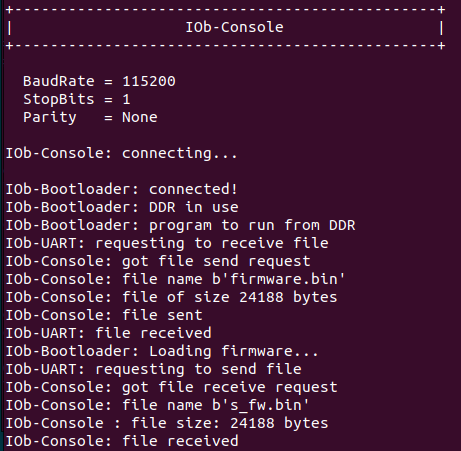
\includegraphics[width=\textwidth]{start_hello_fpga.png}
        \caption{Start of the \enquote{Hello World!} firmware.}
        \label{fig:start_hello_fpga}
    \end{subfigure}
    \hfill
    \begin{subfigure}[b]{0.49\textwidth}
        \centering
        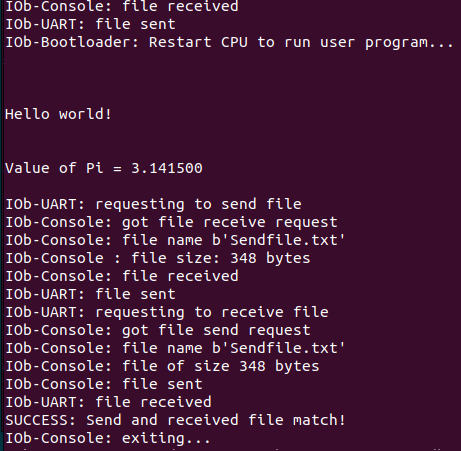
\includegraphics[width=\textwidth]{end_hello_fpga.png}
        \caption{End of the \enquote{Hello World!} firmware.}
        \label{fig:end_hello_fpga}
    \end{subfigure}
    \caption{Running the \enquote{Hello World!} firmware in the FPGA Board.}
    \label{fig:hello_fpga}
\end{figure}

In the tables in \ref{tab:fpga_hello} are the FPGA implementation results for two FPGA families. The author implemented the developed \acrshort{soc} on the kintex Ultrascale AES-KU040-DB-G board and in the CYCLONE V GT-DK. The kintex Ultrascale has an \acrshort{fpga} more capable then the CYCLONE V.

\begin{table}[h]
    \begin{subtable}[h]{0.45\textwidth}
        \centering
        \begin{tabular}{l|l|l|}
            \cline{2-3}
                                              & Authors SoC & \textit{IOb-SoC} \\ \hline
            \multicolumn{1}{|l|}{ALM}         & 10,062      & 9,280            \\ \hline
            \multicolumn{1}{|l|}{FF}          & 12150       & 10020            \\ \hline
            \multicolumn{1}{|l|}{DSP}         & 8           & 3                \\ \hline
            \multicolumn{1}{|l|}{BRAM blocks} & 234         & 352              \\ \hline
            \multicolumn{1}{|l|}{BRAM bits}   & 753,248     & 779,744          \\ \hline
        \end{tabular}
       \caption{Cyclone V GT}
       \label{tab:cyclone_hello}
    \end{subtable}
    \hfill
    \begin{subtable}[h]{0.45\textwidth}
        \centering
        \begin{tabular}{l|l|l|}
            \cline{2-3}
                                            & Authors SoC & \textit{IOb-SoC} \\ \hline
            \multicolumn{1}{|l|}{LUTs}      & 21226       & 23003            \\ \hline
            \multicolumn{1}{|l|}{Registers} & 23373       & 22588            \\ \hline
            \multicolumn{1}{|l|}{DSPs}      & 10          & 7                \\ \hline
            \multicolumn{1}{|l|}{BRAM}      & 39.5        & 34.5             \\ \hline
        \end{tabular}
        \caption{Kintex Ultrascale}
        \label{tab:kintex_hello}
     \end{subtable}
     \caption{FPGA results for \enquote{Hello World!} program using external memory.}
     \label{tab:fpga_hello}
\end{table}

The author obtained the values in table \ref{tab:fpga_hello} while using the \acrshort{soc} with the external memory. When synthesising the \acrshort{soc} the user is able to define whether he wants to use external memory with the \enquote{RUN\_EXTMEM} flag. If \enquote{RUN\_EXTMEM=1} then a memory controller will be synthesised alongside the developed \acrshort{soc} and loaded onto the \acrshort{fpga}. The memory controller is hardware logic written in Verilog and specific to the \acrshort{fpga} where the \acrshort{soc} is running. In order to better understand the resources utilization the author decided to compare the resources uses when running the \enquote{Hello World!} firmware from the internal memory. The resources without the memory controller are in tables \ref{tab:fpga_hello_int_mem}.

\begin{table}[h]
    \begin{subtable}[h]{0.45\textwidth}
        \centering
        \begin{tabular}{l|l|l|}
            \cline{2-3}
                                              & Authors SoC & \textit{IOb-SoC} \\ \hline
            \multicolumn{1}{|l|}{ALM}         & 3,687       & 1,542            \\ \hline
            \multicolumn{1}{|l|}{FF}          & 4707        & 1214             \\ \hline
            \multicolumn{1}{|l|}{DSP}         & 8           & 3                \\ \hline
            \multicolumn{1}{|l|}{BRAM blocks} & 56          & 38               \\ \hline
            \multicolumn{1}{|l|}{BRAM bits}   & 408,800     & 296,960          \\ \hline
        \end{tabular}
       \caption{Cyclone V GT}
       \label{tab:cyclone_hello_int_mem}
    \end{subtable}
    \hfill
    \begin{subtable}[h]{0.45\textwidth}
        \centering
        \begin{tabular}{l|l|l|}
            \cline{2-3}
                                            & Authors SoC & \textit{IOb-SoC} \\ \hline
            \multicolumn{1}{|l|}{LUTs}      & 5457        & 2072             \\ \hline
            \multicolumn{1}{|l|}{Registers} & 4405        & 1074             \\ \hline
            \multicolumn{1}{|l|}{DSPs}      & 7           & 4                \\ \hline
            \multicolumn{1}{|l|}{BRAM}      & 14          & 9                \\ \hline
        \end{tabular}
        \caption{Kintex Ultrascale}
        \label{tab:kintex_hello_int_mem}
     \end{subtable}
     \caption{FPGA results for \enquote{Hello World!} program.}
     \label{tab:fpga_hello_int_mem}
\end{table}

From the tables in \ref{tab:fpga_hello_int_mem} the author can confirm the \textit{VexRiscv} \acrshort{cpu} requires more resources than the \textit{PicoRV32}. Since all components except the \acrshort{cpu} are equal in both \acrshort{soc} the difference in resources is the difference in the \acrshort{cpu}.

\section{Interrupt Routines}
To test the correct functionality of the interrupts in the \acrshort{soc} the author executed the developed \acrshort{clint} testbench. Moreover to test the complete \acrshort{soc} he run the bare-metal firmware created to handled interrupts. The firmware was executed in simulation and implemented in the \acrshort{fpga} Board.

The size of the firmware that testes the interrupt routine is 24364 Bytes. Consequently the only difference in the \acrshort{soc} used on this section tests is the addition of the \acrshort{clint} hardware. The memory size is the same since the \enquote{Hello World!} program and this firmware have similar sizes, both are under 32 KB.

\subsection{Execute CLINT simulation}
After developing the \acrshort{clint} unit the author executed its testbench testing the timer and software interrupts. In figure ... the readers can see a successful simulation of the \acrshort{clint} executing the interrupts.

\begin{figure}[!ht]
    \centering
    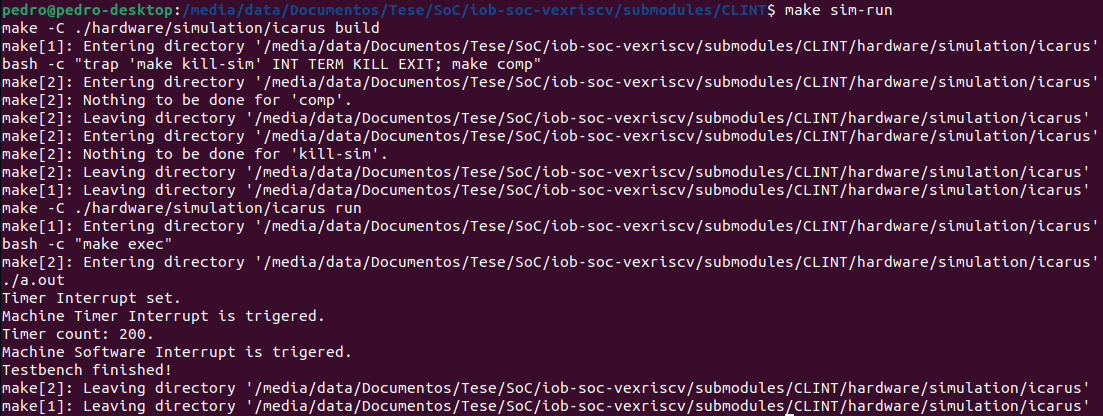
\includegraphics[width=\textwidth]{clint_sim.png}
    \caption{\acrshort{clint} timer and software interrupt simulation.}
    \label{fig:clint_sim}
\end{figure}

\subsection{Execute in simulation}
\begin{figure}[!ht]
    \centering
    \begin{subfigure}[b]{0.49\textwidth}
        \centering
        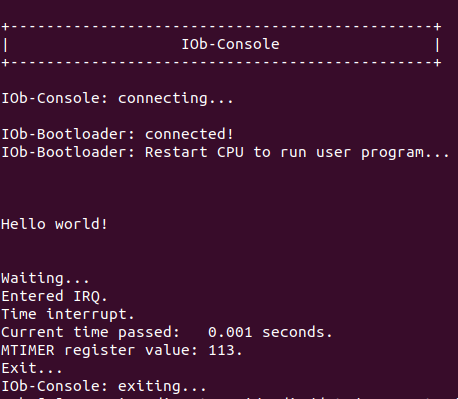
\includegraphics[width=\textwidth]{icarus_int_sim.png}
        \caption{Interrupt routine firmware with \textit{Icarus}.}
        \label{fig:icarus_int_sim}
    \end{subfigure}
    \hfill
    \begin{subfigure}[b]{0.49\textwidth}
        \centering
        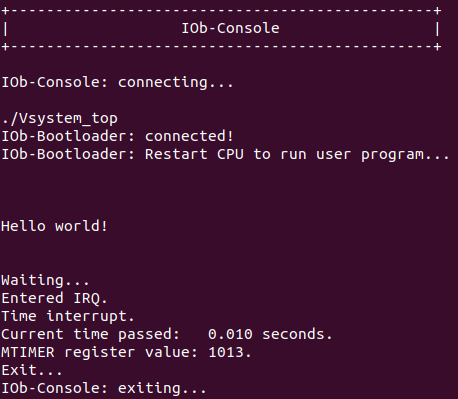
\includegraphics[width=\textwidth]{verilator_int_sim.png}
        \caption{Interrupt routine firmware with \textit{Verilator}.}
        \label{fig:verilator_int_sim}
    \end{subfigure}
    \caption{Running the interrupt routine firmware in the FPGA Board.}
    \label{fig:int_sim}
\end{figure}

\subsection{Execute in the FPGA Board}

\begin{figure}[!ht]
    \centering
    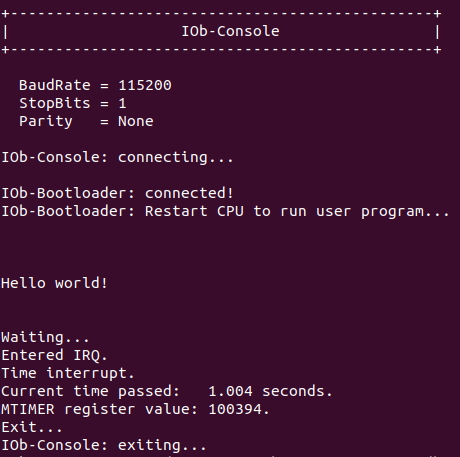
\includegraphics[width=0.49\textwidth]{int_fpga.png}
    \caption{Executing the interrupt routine program on the \acrshort{fpga}.}
    \label{fig:int_fpga}
\end{figure}
% talk 0.004 seconds after it is the time the interrupt handler takes to execute. It is different from the simulation because of the baud rate.

\begin{table}[h]
    \begin{subtable}[h]{0.45\textwidth}
        \centering
        \begin{tabular}{l|l|l|}
            \cline{2-3}
                                              & RUN\_EXTMEM=0 & RUN\_EXTMEM=1 \\ \hline
            \multicolumn{1}{|l|}{ALM}         & 3,883         & 10,257        \\ \hline
            \multicolumn{1}{|l|}{FF}          & 4940          & 12300         \\ \hline
            \multicolumn{1}{|l|}{DSP}         & 8             & 8             \\ \hline
            \multicolumn{1}{|l|}{BRAM blocks} & 56            & 234           \\ \hline
            \multicolumn{1}{|l|}{BRAM bits}   & 408,800       & 753,248       \\ \hline
        \end{tabular}
       \caption{Cyclone V GT}
       \label{tab:cyclone_int}
    \end{subtable}
    \hfill
    \begin{subtable}[h]{0.45\textwidth}
        \centering
        \begin{tabular}{l|l|l|}
            \cline{2-3}
                                            & RUN\_EXTMEM=0 & RUN\_EXTMEM=1 \\ \hline
            \multicolumn{1}{|l|}{LUTs}      & 5729          & 21478         \\ \hline
            \multicolumn{1}{|l|}{Registers} & 4580          & 23545         \\ \hline
            \multicolumn{1}{|l|}{DSPs}      & 7             & 10             \\ \hline
            \multicolumn{1}{|l|}{BRAM}      & 14            & 39.5          \\ \hline
        \end{tabular}
        \caption{Kintex Ultrascale}
        \label{tab:kintex_int}
     \end{subtable}
     \caption{FPGA results for interrupt routine program.}
     \label{tab:fpga_int}
\end{table}


\section{Run/Boot Linux Performance}
\begin{figure}
    \centering
    \begin{subfigure}[b]{0.49\textwidth}
        \centering
        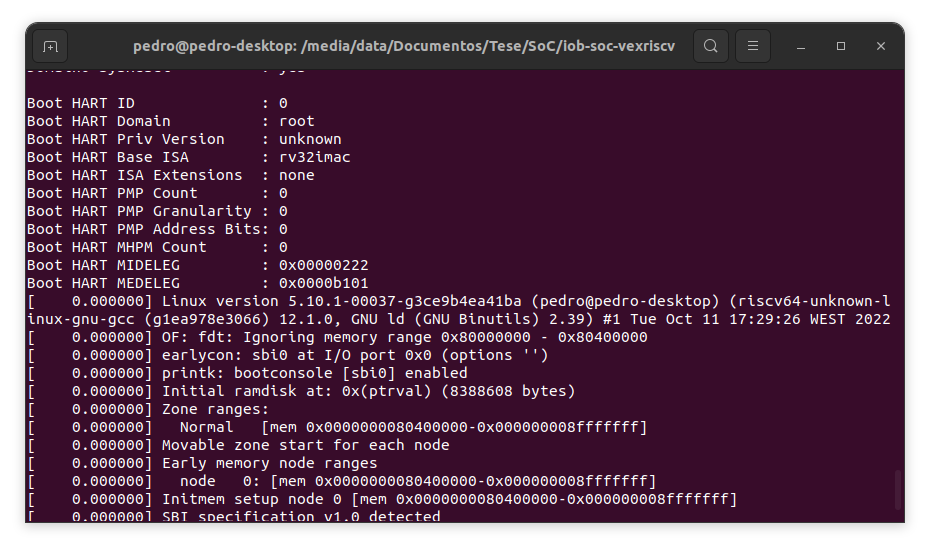
\includegraphics[width=\textwidth]{start_Linux_sim.png}
        \caption{Start of the Linux kernel.}
        \label{fig:start_linux_verilator}
    \end{subfigure}
    \hfill
    \begin{subfigure}[b]{0.49\textwidth}
        \centering
        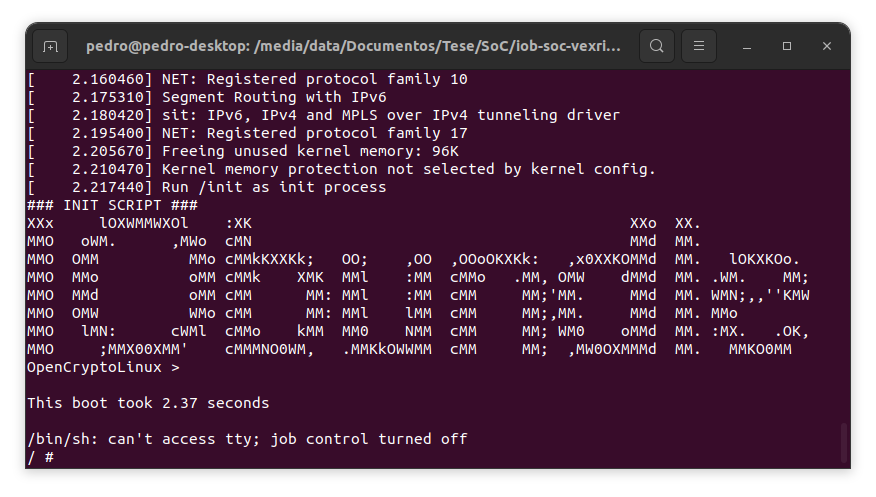
\includegraphics[width=\textwidth]{end_Linux_sim.png}
        \caption{End of Linux kernel boot.}
        \label{fig:end_linux_verilator}
    \end{subfigure}
    \caption{Running Linux with \textit{Verilator}.}
    \label{fig:linux_verilator}
\end{figure}
time that it takes to build a complete OS
real    4m29,570s
user    8m12,039s
sys    0m56,887s



\chapter{Conclusions}
\label{chapter:conclusions}

%%%%%%%%%%%%%%%%%%%%%%%%%%%%%%%%%%%%%%%%%%%%%%%%%%%%%%%%%%%%%%%%%%%%%%%%%%%%%
\section{Achievements}
\label{section:achievements}

% ----------------------------------------------------------------------
\section{Contributed Repositories}
\label{section:contributions}
\begin{itemize}
    \item \textbf{iob-soc}
    \item \textbf{iob-soc-vexriscv}
    \item \textbf{iob-lib}
    \item \textbf{iob-vexriscv}
    \item \textbf{iob-uart16550}
    \item \textbf{iob-clint}
    \item \textbf{iob-plic}
\end{itemize}

% ----------------------------------------------------------------------
\section{Future Work}
\label{section:future}
\begin{itemize}
    \item ethernet
    \item development board with IOb-SoC
\end{itemize}


% ------------------
% |    Appendix    |
% ------------------
\appendix
\cleardoubleoddpage
\pagenumbering{Roman}
\setcounter{page}{11}
\appendix
\chapter{Annex}
% \addchap{Anhang} % kein A vorne (A | Anhang)

\section{Annex 1 - Device Tree Source}
\label{section:annex1}

\begin{lstlisting}[caption={Makefile target to build OpenSBI.}, label=lst:build_opensbi]
/dts-v1/;

/ {
  #address-cells = <1>;
  #size-cells = <1>;
  model = "IOb-SoC, VexRiscv";
  compatible = "IOb-SoC, VexRiscv";
	cpus {
    #address-cells = <0x1>;
    #size-cells = <0x0>;
    timebase-frequency = <100000>;
		CPU0: cpu@0 {
			clock-frequency = <100000000>;
            device_type = "cpu";
			reg = <0x0>;
			status = "okay";
            compatible = "riscv";
			riscv,isa = "rv32imac";
			mmu-type = "riscv,sv32";
			d-cache-block-size = <0x40>;
			d-cache-sets = <0x40>;
			d-cache-size = <0x8000>;
			d-tlb-sets = <0x1>;
			d-tlb-size = <0x20>;
			i-cache-block-size = <0x40>;
			i-cache-sets = <0x40>;
			i-cache-size = <0x8000>;
			i-tlb-sets = <0x1>;
			i-tlb-size = <0x20>;
			tlb-split;
			CPU0_intc: interrupt-controller {
				#interrupt-cells = <1>;
				interrupt-controller;
				compatible = "riscv,cpu-intc";
			};
		};
	};
  memory@80000000 {
    device_type = "memory";
    reg = <0x80000000 0x10000000>;
  };
  chosen {
    bootargs = "rootwait console=hvc0 earlycon=sbi root=/dev/ram0 init=/sbin/init swiotlb=32";
  	linux,initrd-start = <0x81000000>;
  	linux,initrd-end = <0x81800000>; // max 8MB ramdisk image
  };
  soc {
    #address-cells = <1>;
    #size-cells = <1>;
    compatible = "iobundle,iob-soc", "simple-bus";
    ranges;
    clint@60000000 {
      compatible = "riscv,clint0";
      interrupts-extended = <&CPU0_intc 3 &CPU0_intc 7>;
      reg = <0x60000000 0xc0000>;
      reg-names = "control";
    };
    // PLIC needs to be disabeld for tandem verification
    //PLIC0: interrupt-controller@50000000 {
    //  #address-cells = <0>;
    //  #interrupt-cells = <1>;
    //  compatible = "riscv,plic0";
    //  interrupt-controller;
    //  interrupts-extended = <&CPU0_intc 0xb>;
    //  reg = <0x50000000 0x4000000>;
    //  riscv,max-priority = <7>;
    //  riscv,ndev = <0xa>;
    //};
    // Specifying the interrupt controller in the devicetree is not necessary.
    // Furthermore, the IRQ 65535 will cause a `hwirq 0xffff is too large` during
    // Linux boot (occured with mainline linux 5.14.0).
    uart@40000000 {
      compatible = "ns16550a";
      reg = <0x40000000 0x1000>;
      clock-frequency = <100000000>;
      current-speed = <115200>;
      //interrupt-parent = < &PLIC0 >;
      interrupts = <1>;
      reg-shift = <2>; // regs are spaced on 32 bit boundary
      reg-io-width = <4>; // only 32-bit access are supported
    };
  };
};
\end{lstlisting}


\section{Annex 2}
Annex 2


% ----------------------
% |    Bibliography    |
% ----------------------
\printbibliography
% \printbibheading[title=Literatur]
% \printbibliography[heading=subbibliography, type=online, title={Online}]
% \printbibliography[heading=subbibliography, type=book, title={Literatur}]
% \printbibliography[heading=subbibliography,title={Der ganze Rest},nottype=online,notkeyword=Norm,notkeyword=sekundaer]

\end{document}
